%%%%%%%%%%%%%%%%%%%%%%%%%%%%%%%%%%%%%%%%%%%%%%%%%%%%%%%%%%%%%%%%%%%%%%%%%%%%%%%%
%2345678901234567890123456789012345678901234567890123456789012345678901234567890
%        1         2         3         4         5         6         7         8

%\documentclass[letterpaper, 10 pt, conference]{ieeeconf}  % Comment this line out
                                                          % if you need a4paper
\documentclass[a4paper, 10pt, conference]{ieeeconf}      % Use this line for a4
                                                          % paper

\IEEEoverridecommandlockouts                              % This command is only
                                                          % needed if you want to
                                                          % use the \thanks command
\overrideIEEEmargins
% See the \addtolength command later in the file to balance the column lengths
% on the last page of the document

% The following packages can be found on http:\\www.ctan.org
%\usepackage{graphics} % for pdf, bitmapped graphics files
%\usepackage{epsfig} % for postscript graphics files
%\usepackage{mathptmx} % assumes new font selection scheme installed
%\usepackage{times} % assumes new font selection scheme installed
%\usepackage{amsmath} % assumes amsmath package installed
%\usepackage{amssymb}  % assumes amsmath package installed

\usepackage{epsf,graphicx}
\usepackage{latexsym,amssymb}
\usepackage{setspace,cite}
\usepackage{graphicx}
\usepackage{caption}
\usepackage{subcaption}
\usepackage{hyperref}
\usepackage[]{algorithm2e}
\usepackage{amsmath}
\usepackage{gensymb}
\usepackage[usenames,dvipsnames]{xcolor}
\usepackage{tikz}
\usepackage{listings}
\usepackage{adjustbox}




\title{\LARGE \bf
Automatic behavioral adaptation based on engagement assessment in child-robot interaction
}

\author{Fernando Garcia, S\'everin Lemaignan% <-this % stops a space
\thanks{F. Garcia is with Computer Human Interaction Learning and Instruction Laboratory, EPFL (CH).
        {\tt\small fernando.garcia@epfl.ch }}
}

\begin{document}

\maketitle
\thispagestyle{empty}
\pagestyle{empty}


%%%%%%%%%%%%%%%%%%%%%%%%%%%%%%%%%%%%%%%%%%%%%%%%%%%%%%%%%%%%%%%%%%%%%%%%%%%%%%%%
\begin{abstract}

Sustaining long-term interventions in a human-robot interaction scenario with an engaged user requires a system able to provide a suitable response depending on the context of the situation. It becomes a must to capture the significant \textit{passive} information provided by the user during the interaction that can be used to assess user's engagement. Furthermore, this evaluation can also be used to provide a variety of behavioral responses according to the interaction particularities. Here, an automatic behavioral adaptation model based on engagement assessment in the context of the CoWriter project is proposed. Several methods for face feature acquisition on real time has been implemented and tested with children. The results obtained are validated with a ground truth acquired during the sessions through a visual assessment from two observers. Such results has shown significance in the proximity to the field of interaction as an indicator of child's engagement in the activity. 

\end{abstract}


%%%%%%%%%%%%%%%%%%%%%%%%%%%%%%%%%%%%%%%%%%%%%%%%%%%%%%%%%%%%%%%%%%%%%%%%%%%%%%%%
\section{INTRODUCTION}

The CoWriter project aims to explore how a robot can help with the acquisition of writing skills. This project especially targets children, as handwriting difficulties in children at an early age often negatively affects their academic performance \cite{christensen2005role} in addition to their self-esteem being adversely affected \cite{malloy1995handwriting}. The use of robots in handwriting education presents an opportunity for the children to interact with an embodied, physical agent as part of the learning experience as well as the potential to engage the child in meta-cognition through the learning by teaching paradigm \cite{palinscar1984reciprocal}.

A first prototype implemented by D.Hood et al. \cite{hood2015children} has shown good results in terms of robustness and functionality. The current system is based on a Nao humanoid robot with limited motion capabilities and thus, linked with a tablet as IO device using ROS. The tactile screen allows both the collection of user's shape demonstrations but also the display of the simulated handwriting computed using a PCA based algorithm \cite{hood2015children}.

Sustaining long-term interventions in the educational context described trying to maximize the duration of the interactions and across several sessions at a high engagement level, becomes an important issue. Indeed, setting a social bond through the expression of feelings, emotions and adaptive gestures may be useful to keep a higher engagement level. These expressions are very important in interactions and the forming of social relationships \cite{butler2003social}\cite{mcneill1992hand}. Hopefully, several studies, among them \cite{leite2012modelling} show that empathy facilities interaction in robot-child interaction, showing that human-based expressions can be successfully implemented by robots. Actually, based on the previous statements, \cite{beran2011understanding} established that the expressive behavior of children can be influenced positively by adapting the emotion expression of their robotic interaction partner.

\subsection{The engagement in interaction}
Until recently, engagement was defined vaguely as a cognitive, affective (specifically intrinsic motivation), and behavioral state of interaction with a computer application that "makes the user want to be there" \cite{ASI:ASI21229}. Engaging interactions were thought to involve attention, intrinsic interest, interactivity, perceived control and choice, functionality and motivation. This collection of attributes was derived from studies carried out in multiple disciplines (i.e., education, e-commerce, human-computer interaction, etc.) with varied applications, including educational multimedia, presentation software and video games.

\subsection{Models of behavior}

In emotion research field there are two main established approaches. The first of them is based on distinguishing several basic emotions that implicitly assumes a discretization. The second one considers an emotion to be a combination of two concepts: valence and arousal. Arousal could be define as how exiting the emotion is, having several degrees of intensity whereas valence, would be how positive or negative the emotion is perceived.
If the robot reacts directly from the environment, then it is functional but if it reacts according to its internal state becomes biologically inspired. Studies like \cite{schulte1999spontaneous} employs a state-machine based solution, but the recent tendency is to go towards a long-term interaction driven by the existence of an internal state \cite{hirth2011towards} \cite{canamero2001show}.
Tielman et al. for instance, proposed a model \cite{tielman2014adaptive} based on both by separation between gestures and emotion externalization. Recent works \cite{lim2014mei} focus more on the feature acquisition from the environment. Features often related with the voice such as pitch volume or intensity.

Here, we present a functional approach based on a valence and arousal model for automatic adaptation behavior based on possible engagement features extracted from the user. 
\section{Hypothesis}
In this work it has been hypothesize that the engagement assessment within the CoWriter context can be detected through the measurement of the following variables on real time: Quantity of movement (QoM), proximity to the field of interaction (FoI), saliency and focus of attention (FoA) through gaze direction. In addition, and based on the measurements of this features, an automatic behavioral adaptation model is proposed for Nao.

\section{Approach}
The main approach of this contribution consist on implementing a new non-engaging activity, a simple \textit{story telling}, in addition to the current engaging activity, \textit{writing}. Through the measurement of the focus of attention, the proximity to the FoI, the QoM and the saliency of several features during the execution of both tasks, it has been possible to detect when a child is engaged or not. Furthermore, all these features have been used, together with a few more measurements such as time spend in the activity and the number of word repetitions performed, to adapt in real time the behavior of the Nao humanoid robot according to the situation context.

In this way, the model presented has been divided in three different blocks: The vision module, the emotion manager and the action manager. As their names indicate, the vision module contains the face tracking and the methods used for visual feature extraction. The emotion manager weights the incoming feature information providing a response towards an specific behavior. Finally, the action manager transforms this result into a behavior expression.

\subsection{Vision module}
Some of the candidate features need a robust real-time 2D face pose estimation. \textit{Dlib} library has allowed to track precisely even with partial occlusions or in poor light conditions relevant face landmarks.

\subsubsection{Proximity to the field of interaction}
Back posture has been proved to be a reliable indicator of user's engagement \cite{d2007posture} \cite{castellano2009detecting}. We believe that this is directly correlated with the proximity towards FoI composed, in this case, by Nao and a tablet. In order to be estimated, it is necessary to compute the middle point between the eyes because it decreases the variability due to the movement like in equation \ref{eq:proximity}.

\small
\begin{equation} \label{eq:proximity}
up(x,y) = \left (\frac{eye_{L}(x)-eye_{R}(x)}{2}, \frac{eye_{L}(y)-eye_{R}(y)}{2}\right )
\end{equation}
\normalsize

Then, the distance in the vertical line of the face can be computed using $ up(x,y) $ and $ chin(x,y)$. Both measurements combined provide the size of the head and thus, a distance measurement with respect to the camera can approximated.

\subsubsection{Quantity of movement}
It is captured and kept during the interaction. In order, to obtain the movement from the scene, several methods has been tested being selected optical-flow as less sensitive to image noise than point-wise methods. The algorithm finds the most prominent corners in the image computing the corner Minimum Eigenvalue as described in \cite{shi1994good}, which stores the minimal eigenvalue of a block size neighborhood \textit{S(p)}, that is, $ \min(\lambda_1, \lambda_2) $ in terms of the following equation:

\begin{equation}
M =  \begin{bmatrix} 
		\sum _{S(p)}(dI/dx)^2 &  \sum _{S(p)}(dI/dx dI/dy)^2  \\ 
		\sum _{S(p)}(dI/dx dI/dy)^2 &  \sum _{S(p)}(dI/dy)^2 
	 \end{bmatrix}
\end{equation} 

where the derivatives are computed using the \textit{Sobel} operator. After that, it finds the minimum eigenvalue of \textit{M} and stores them.

Once the relevant points are detected, the second step is to calculate the flow from these points. The technique used is based on Lucas-Kanade method with pyramids\cite{bouguet2001pyramidal} which assumes that the flow is essentially constant in a local neighborhood of the pixel under consideration and solves the basic optical flow equations for all the pixels in that neighborhood by the least squares criterion. Being the equations formulated as in point \ref{lucasKanade}.

\begin{equation} \label{lucasKanade}
\resizebox{.9\hsize}{!}{$A =  \left( \begin{array}{cc}
	I_x(q_1) & I_x(q_1) \\
	I_x(q_1) & I_x(q_1) \\
	\colon & \colon  \\
	I_x(q_n) & I_x(q_n)
	\end{array} \right),
\qquad  
v =  \left( \begin{array}{cc}
		V_x  \\
		V_y \\
	\end{array} \right),
\qquad	 	 
b =  \left( \begin{array}{c}
	 		-I_t(q_1)\\
	 		-I_t(q_2)\\
	 		\colon \\
	 		-I_t(q_n)\\
	 \end{array} \right)$}
\end{equation}

This system has more equations than unknowns and thus it is usually over-determined. So, needs to be reformulated as shown in equation \ref{lucasKanade1}. 

\begin{equation} \label{lucasKanade1}
A^TAv = A^Tb
\qquad
\Rightarrow
\qquad
v=(A^TA)^{-1}A^Tb
\end{equation}

\subsubsection{Focus of attention}
The FoA factor is defined by the gaze direction. It has been computed using a simple but effective method through the landmark positions.

First, it is necessary to compute the length of the segments between the right and the left face sides ($ side_R $ and $ side_L $, respectively) with respect to the nose, $ d(nose,side_R) $ and $ d(nose,side_L) $, as well as the distance between both sides, $ d(side_R,side_L) $. So, it results in equation \ref{eq:estwest},

\begin{equation} \label{eq:estwest}
horizontal = \frac{d(nose,side_R)-d(nose,side_L)}{d(side_R,side_L)}
\end{equation}

where the result is normalized in the range $ [-1,1] $. A value greater than a threshold of 0.3 indicates \textit{left} as gaze direction, whereas lower than -0.3 indicates \textit{right} direction.

Second, we perform a similar operation to detect when a user is looking up or down. It is necessary to calculate the projection of the nose position in the \textit{horizontal} segment that goes from $ side_R $ to $side_L$ like in equations \ref{eq:projection} and \ref{eq:projection1}.

\begin{equation}\label{eq:projection}
\resizebox{.9\hsize}{!}{$d_{proj} = d(nose,side_R) \cdot \left(\frac{horizontal}{d(nose,side_R)} + d(nose,side_L)\right )$}
\end{equation}

\begin{equation} \label{eq:projection1}
\resizebox{.9\hsize}{!}{$proj(x,y) = \frac{P_{side_R}(x,y)+(P_{side_L}(x,y)-P_{side_R}(x,y))\cdot d_{proj}}{horizontal}$}
\end{equation}

Then, we can compare if the height of $ proj(x,y) $ is greater or lower than the nose position with a certain tolerance. If it is the case, the user is looking up or down respectively. Finally, if none of the directions are satisfied, we assume that the user is looking straight at the robot.


\subsubsection{Saliency}
The \textit{saliency} is a concept that is related with the changes on the current state of the scene. Events such as a new person detected in the scene as well as quick movements after a quiet period or vice-versa, are considered as a saliency. The algorithm implemented for this detection was the Exponential Moving Average (EMA), defined in equation \ref{eq:EMA},

\begin{equation} \label{eq:EMA}
 t > 1,\ \    S_{t} = \alpha \cdot Y_{t} + (1-\alpha) \cdot S_{t-1}
\end{equation}

where the coefficient $ \alpha $ represents the degree of weighting decrease, a constant smoothing factor. A higher $ \alpha $ discounts older observations faster. The $ Y_t $ is the value at a time period \textit{t} and $ S_t $ is the value of the EMA at any time period \textit{t}.

Once the EMA $S_t$ value is computed, the distance with respect to the previous, $S_{t-1}$ needs to be calculated for each kind of event (gaze, proximity...) as shown in equation \ref{eq:EMA2}.

\begin{equation} \label{eq:EMA2}
d = \frac{(S_t - S_{t-1})^2}{\epsilon + (S_t + S_{t-1})^2 }
\end{equation}

As a result, when a high quantity of movement is captured after a period of low movement, a new face is detected, or the proximity changes in great manner the EMA value increases.

\subsection{Emotion manager}
This node is responsible for the vectorization of the incoming information from the \textit{vision} node and eventually, the computation of the correspondent valence and arousal values. Furthermore, besides the features extracted from the \textit{vision} module, there are additional ones such as; the time spend in the activity or the number of repetitions that have an influence in the resulting vectorization of the current state (see figure \ref{fig:vectMap}). The summary of the features used, the direction of the correspondent vectors (valence, arousal) assuming an initial point $ (0,0) $, the weight of them in the final computation, as well as the features that are used for the engagement assessment are shown in table \ref{tab:cues}.

\begin{table}[h!]
\small
\centering
\begin{tabular}{l|c|c|c|c}
 \textbf{Features}   & \textbf{Valence}  & \textbf{Arousal}  & \textbf{Weight} & \textbf{Eng}\\ \hline	
 \textit{QoM}  	  		  	 &   -1 	&    1 	& 14\% &   +  \\ \hline
 \textit{Proximity FoI}    	  	 &   1  &    1	& 7\%  &   +  \\ \hline
 \textit{Saliency}	  	  	 &   0 	    &    1 	& 7\%  &   +  \\ \hline
 \textit{Gaze: robot contact} 	 &   1	&    1 	& 5\%  &   +  \\ \hline
 \textit{Gaze: other directions} & -1	&   -1  & 5\%  &   +  \\ \hline
 \textit{Smiling}	  	  	 &   1 	    &    1 	& 60\% &      \\ \hline
 \textit{Time activity}	  	 &   -1	    &   -1 	& 1\%  &      \\ \hline
 \textit{Number repetitions} &   -1 	&   -1	& 1\%  &       	

\end{tabular}
\caption{Summary of the features in valence, arousal, weight and engagement assessment (Eng)}
\label{tab:cues}
\end{table}

 \begin{figure}[!htb]
	\centering
	\begin{tikzpicture}[>=latex]

		\node[inner sep=0pt] (xtion) at (0,0) {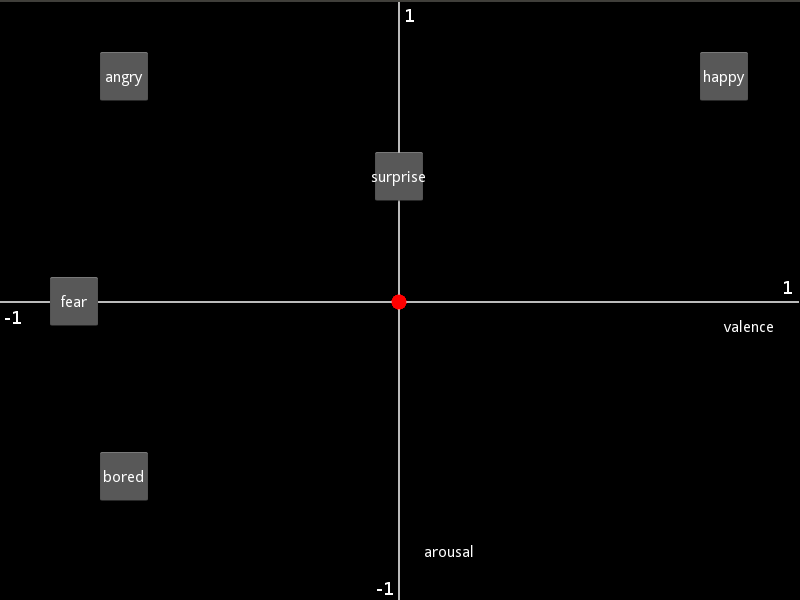
\includegraphics[width=.45\textwidth]{../dissertation/figures/vectMap.png}};

		\draw[->, color=green, thick] (0,0) -- (1.5,1);
		\draw[->, color=yellow, thick] (0,0) -- (0,0.9);
		\draw[->, color=blue, thick] (0,0) -- (-0.75,-0.5);
		\draw[->, color=red, thick] (0,0) -- (-1,0.75);
		\draw[red,fill=red] (0,0) circle (.8ex);
		
		\draw[white, thick,dashed] (0,2.5) ellipse (0.75cm and 0.25cm);
		\node[white, text width=2cm] at (0.7,2.45) {\tiny
		Saliency
		};
		
		\draw[white, thick,dashed] (-1.8,-1.2) ellipse (1cm and 0.75cm);
		\node[white, text width=2cm] at (-1.4,-1.2) {\tiny
		Time activity
		
		Number repetitions		
		Ignoring
		};
		
		\draw[white, thick,dashed] (2.2,1.8) ellipse (1cm and 0.6cm);
		\node[white, text width=1.2cm] at (2.4,1.8) {\tiny
		Smiling
		
		Eye contact				
		Proximity
		};
		
		\draw[white, thick,dashed] (-2.4,1.5) ellipse (0.75cm and 0.25cm);
		\node[white, text width=2cm] at (-1.8,1.45) {\tiny		
		High QoM	
		};
	\end{tikzpicture}
    \caption{Valence and arousal map with features in \textit{[-1,1]}.}
    \label{fig:vectMap}
\end{figure}

The direction of the marker that defines the current behavior (see red dot in figure \ref{fig:vectMap}) depends on the fusion of all different features with their respective weights. The formula that computes the resulting valence and arousal values provided to the action node is shown in \ref{eq:weight}.

\begin{equation}\label{eq:weight}
 \vec{P_{t}}(val,aro) = \sum_{i=1}^N\vec{F}_{i}(val,aro) \cdot w_i
\end{equation}

where $\vec{P_{t}}(val,aro)$ is the vector that defines the behavior at time \textit{t} encoded by valence and arousal values in range \textit{[-1,1]}. It is based on the combination of all vector features $ \vec{F}_{i} $ multiplied by their respective weights \textit{w}.

\begin{figure*}
        \centering        
        \begin{subfigure}[b]{0.18\textwidth}
                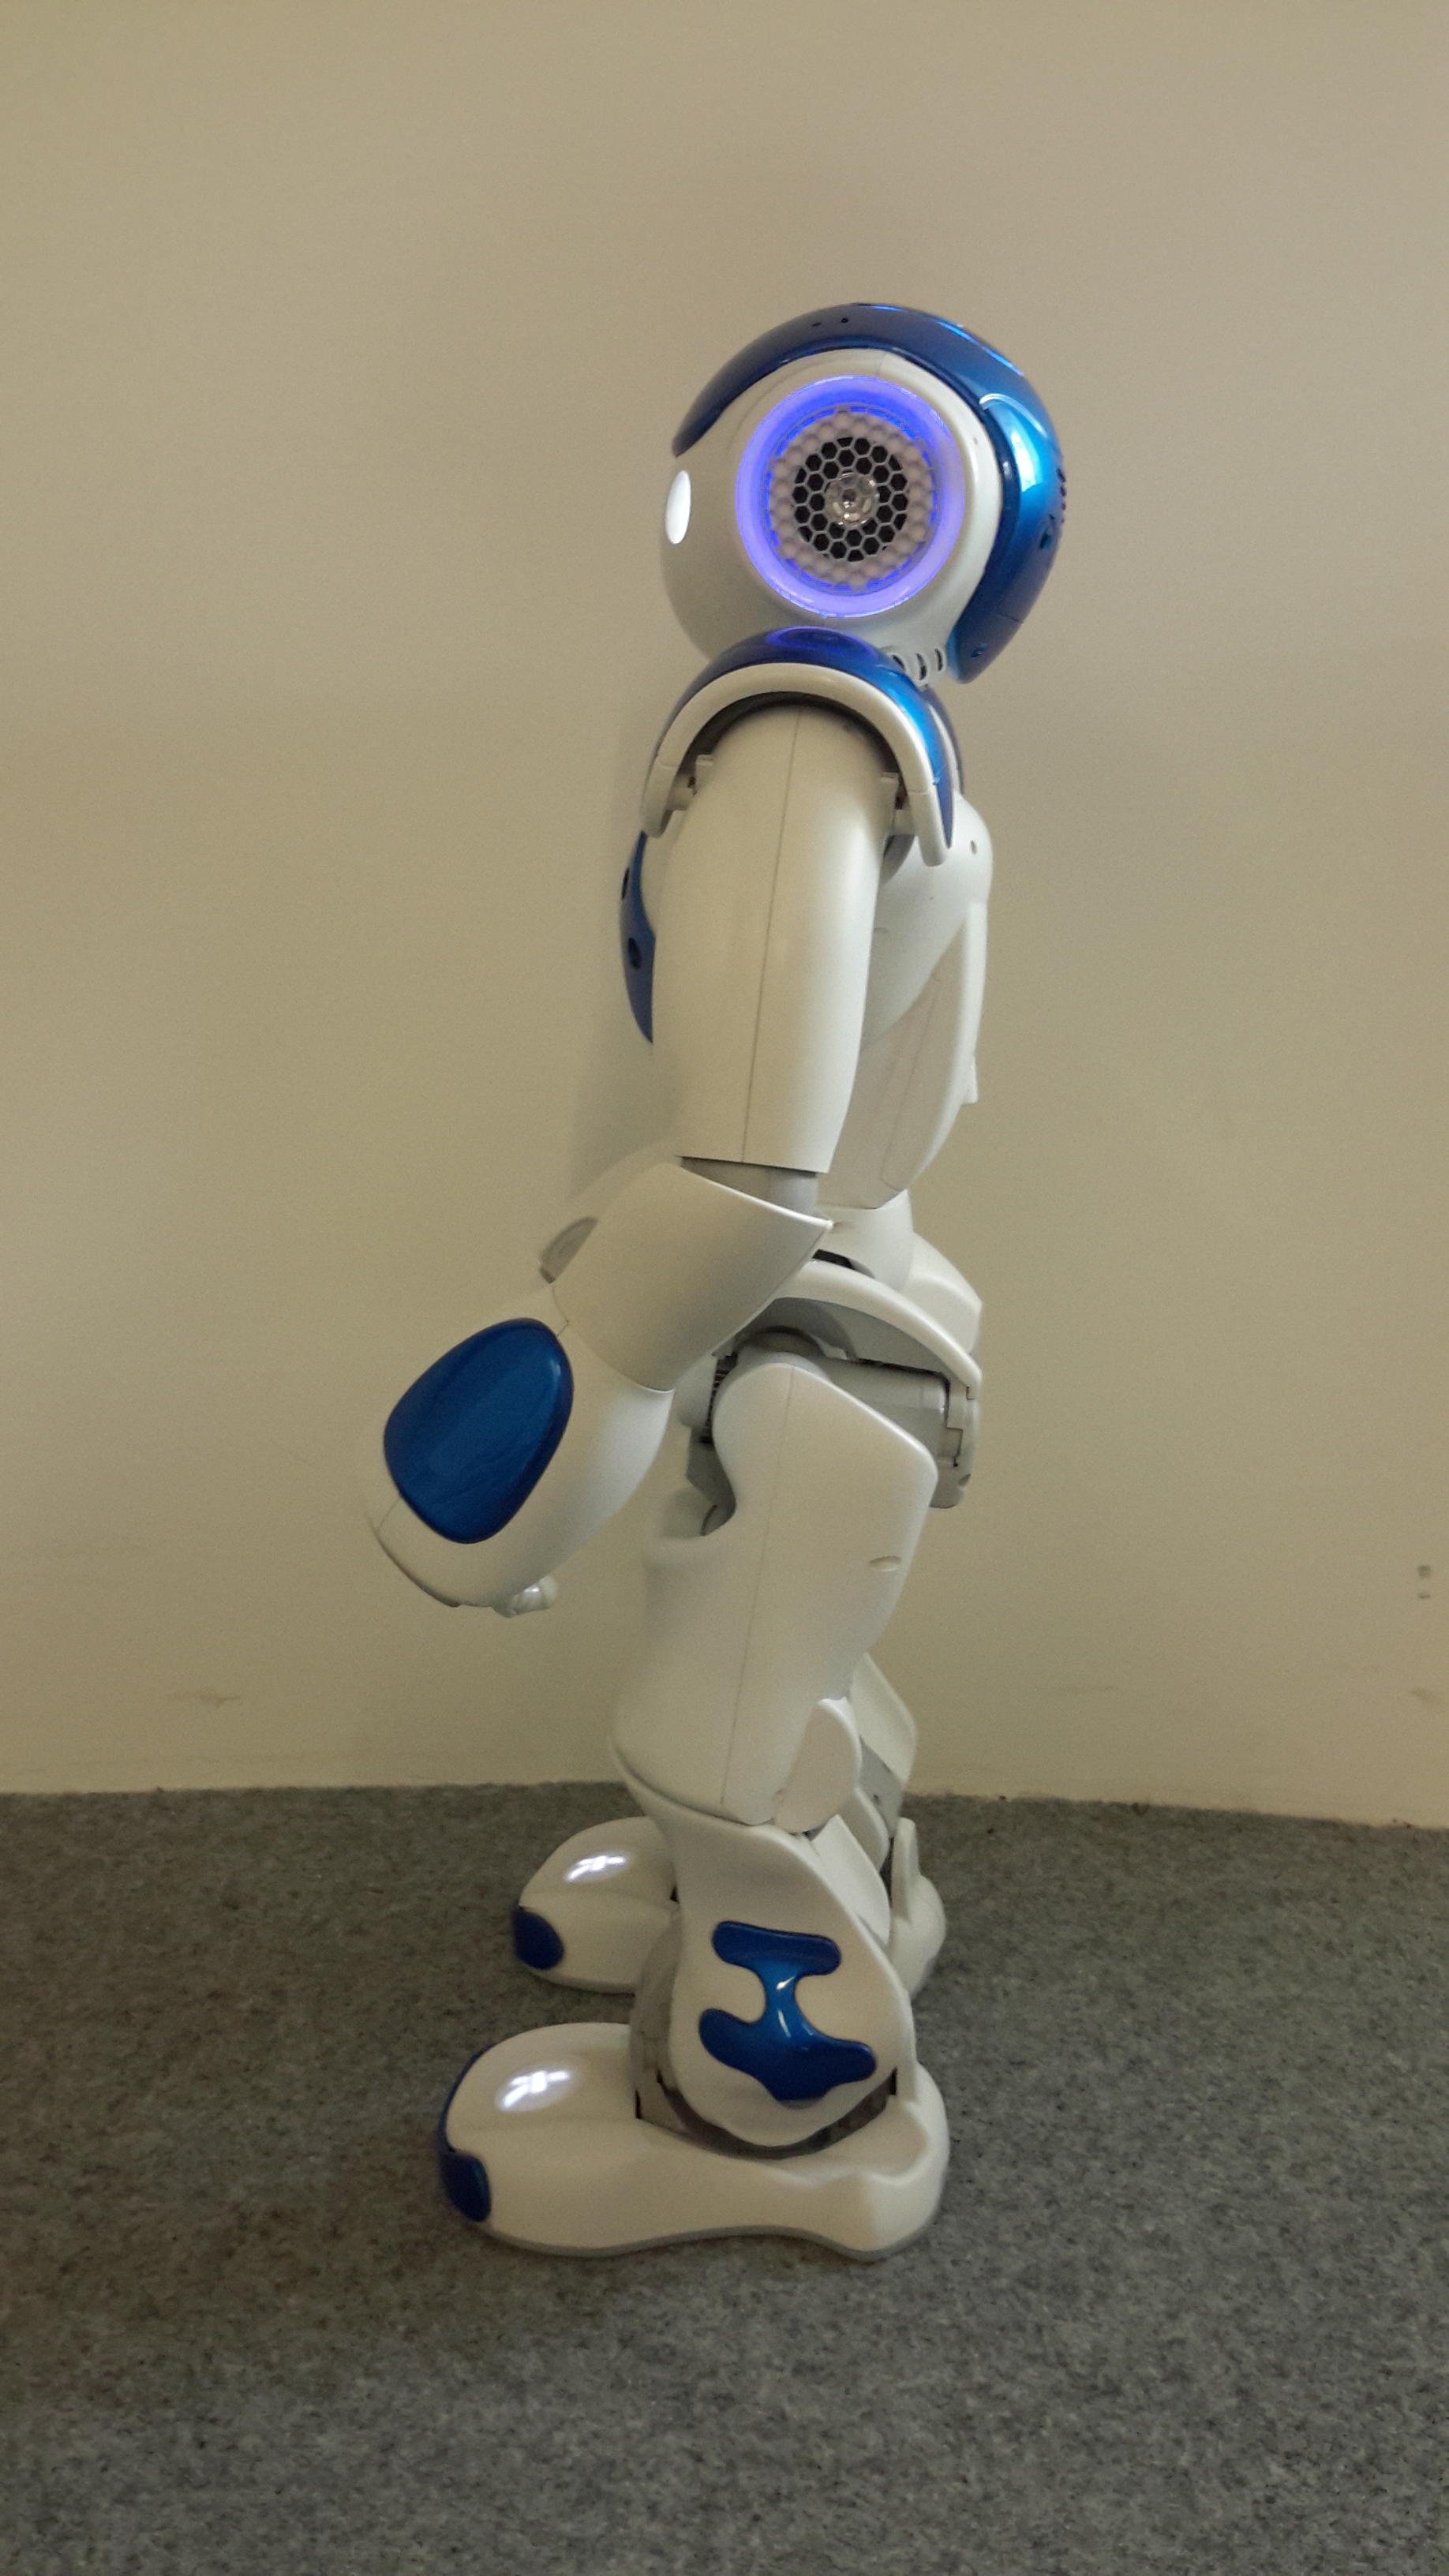
\includegraphics[width=\textwidth]{../dissertation/figures/neutral.jpg}
                \caption{Neutral}
                \label{fig:neutral}
        \end{subfigure}
        ~ %add desired spacing between images, e. g. ~, \quad, \qquad, \hfill etc.
          %(or a blank line to force the subfigure onto a new line)
        \begin{subfigure}[b]{0.18\textwidth}
                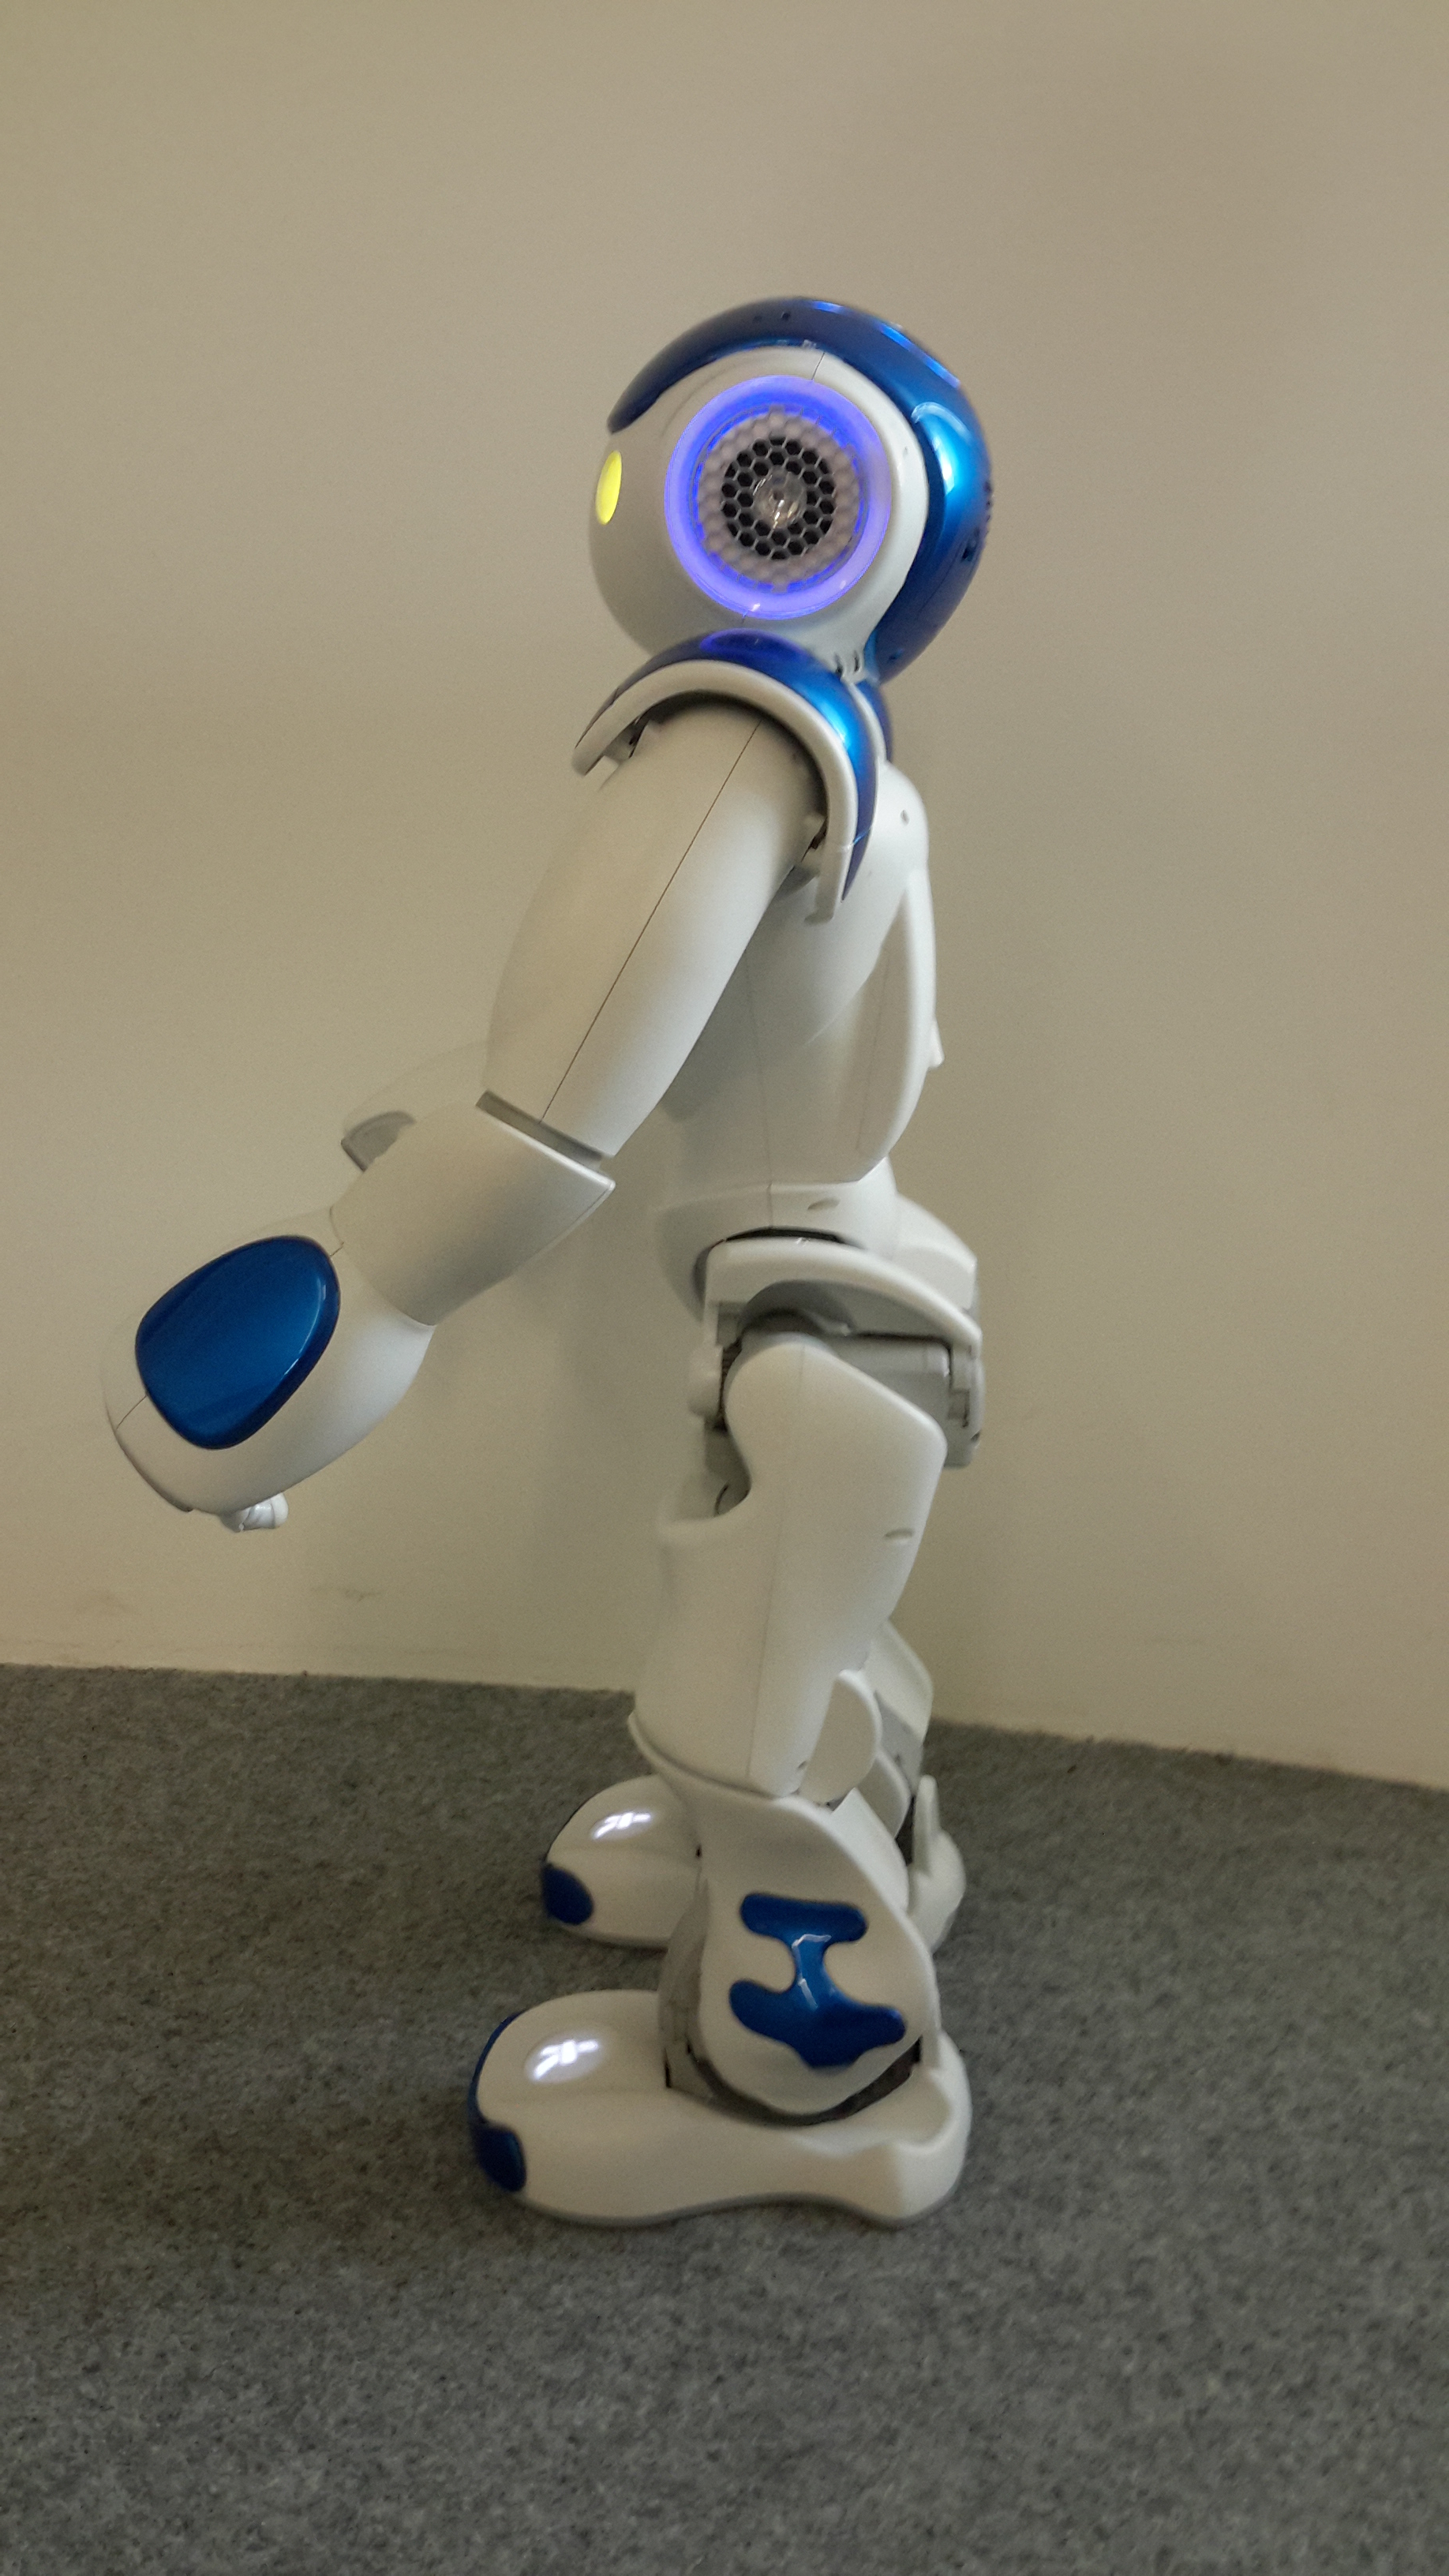
\includegraphics[width=\textwidth]{../dissertation/figures/happy.jpg}
                \caption{Happy}
                \label{fig:happy}
        \end{subfigure}%
        ~ %add desired spacing between images, e. g. ~, \quad, \qquad, \hfill etc.
          %(or a blank line to force the subfigure onto a new line)
        \begin{subfigure}[b]{0.18\textwidth}
                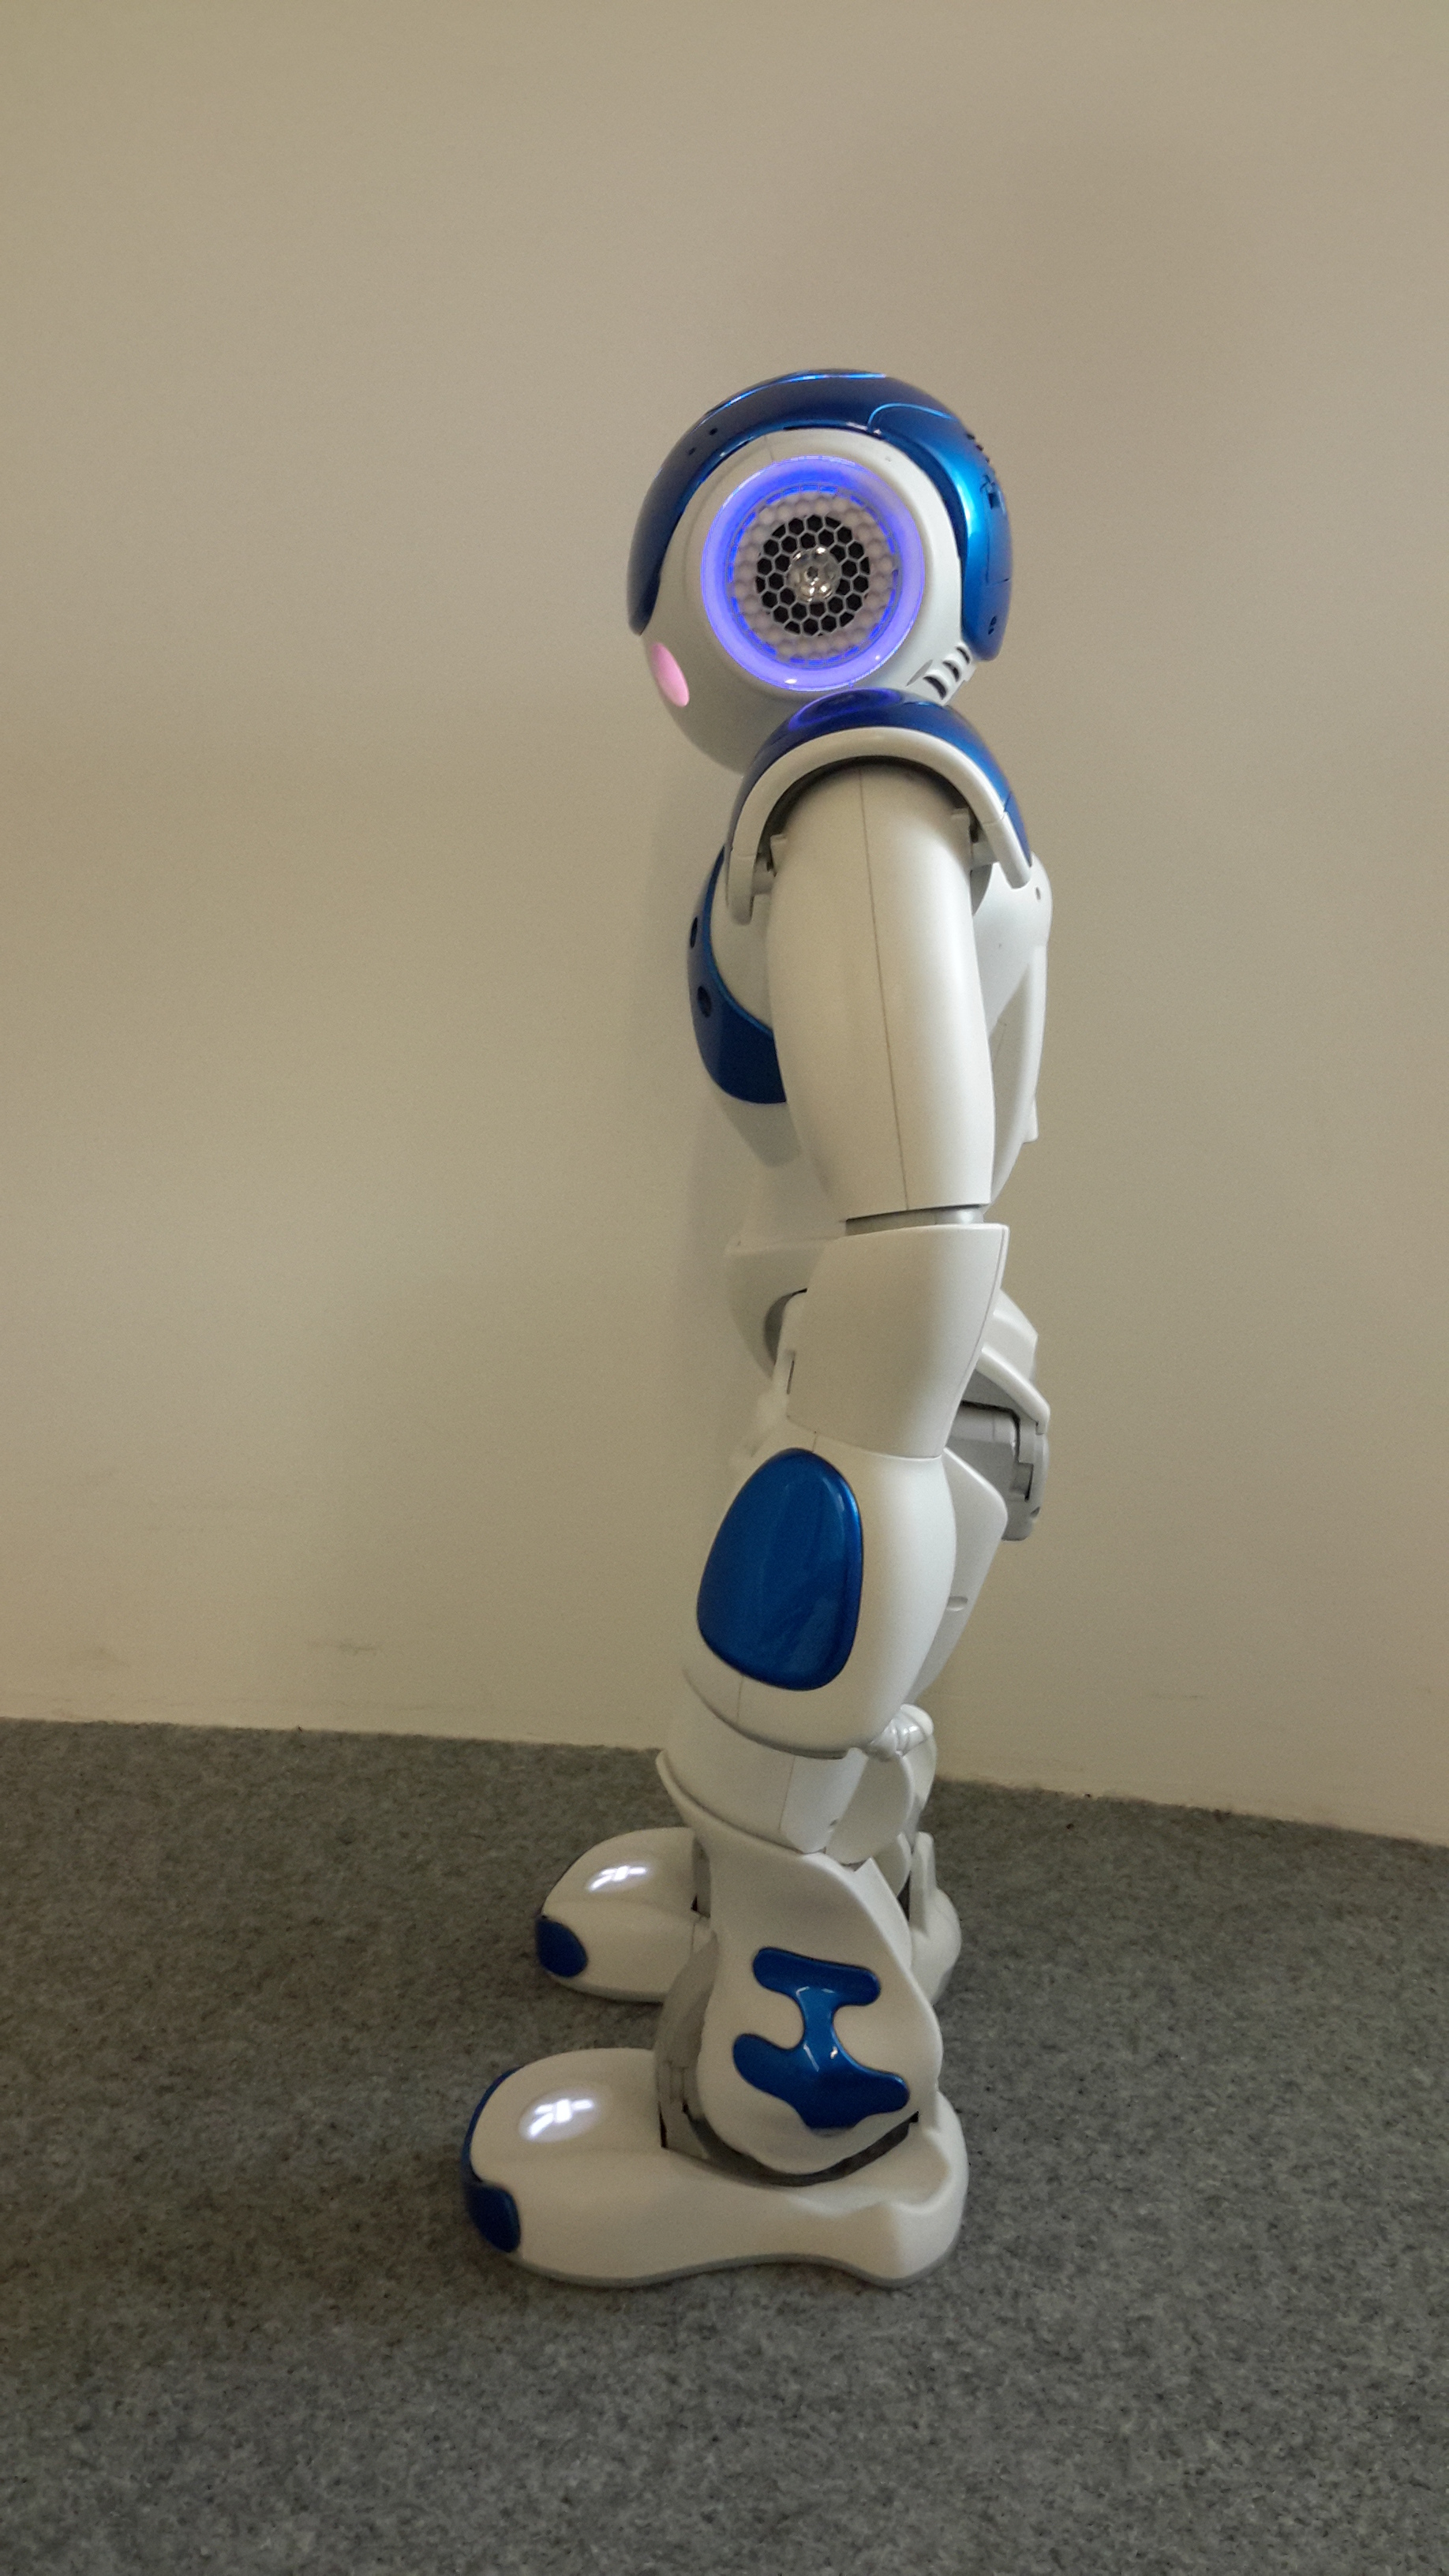
\includegraphics[width=\textwidth]{../dissertation/figures/sad.jpg}
                \caption{Sad}
                \label{fig:sad}
        \end{subfigure}
        ~ %add desired spacing between images, e. g. ~, \quad, \qquad, \hfill etc.
          %(or a blank line to force the subfigure onto a new line)
        \begin{subfigure}[b]{0.18\textwidth}
                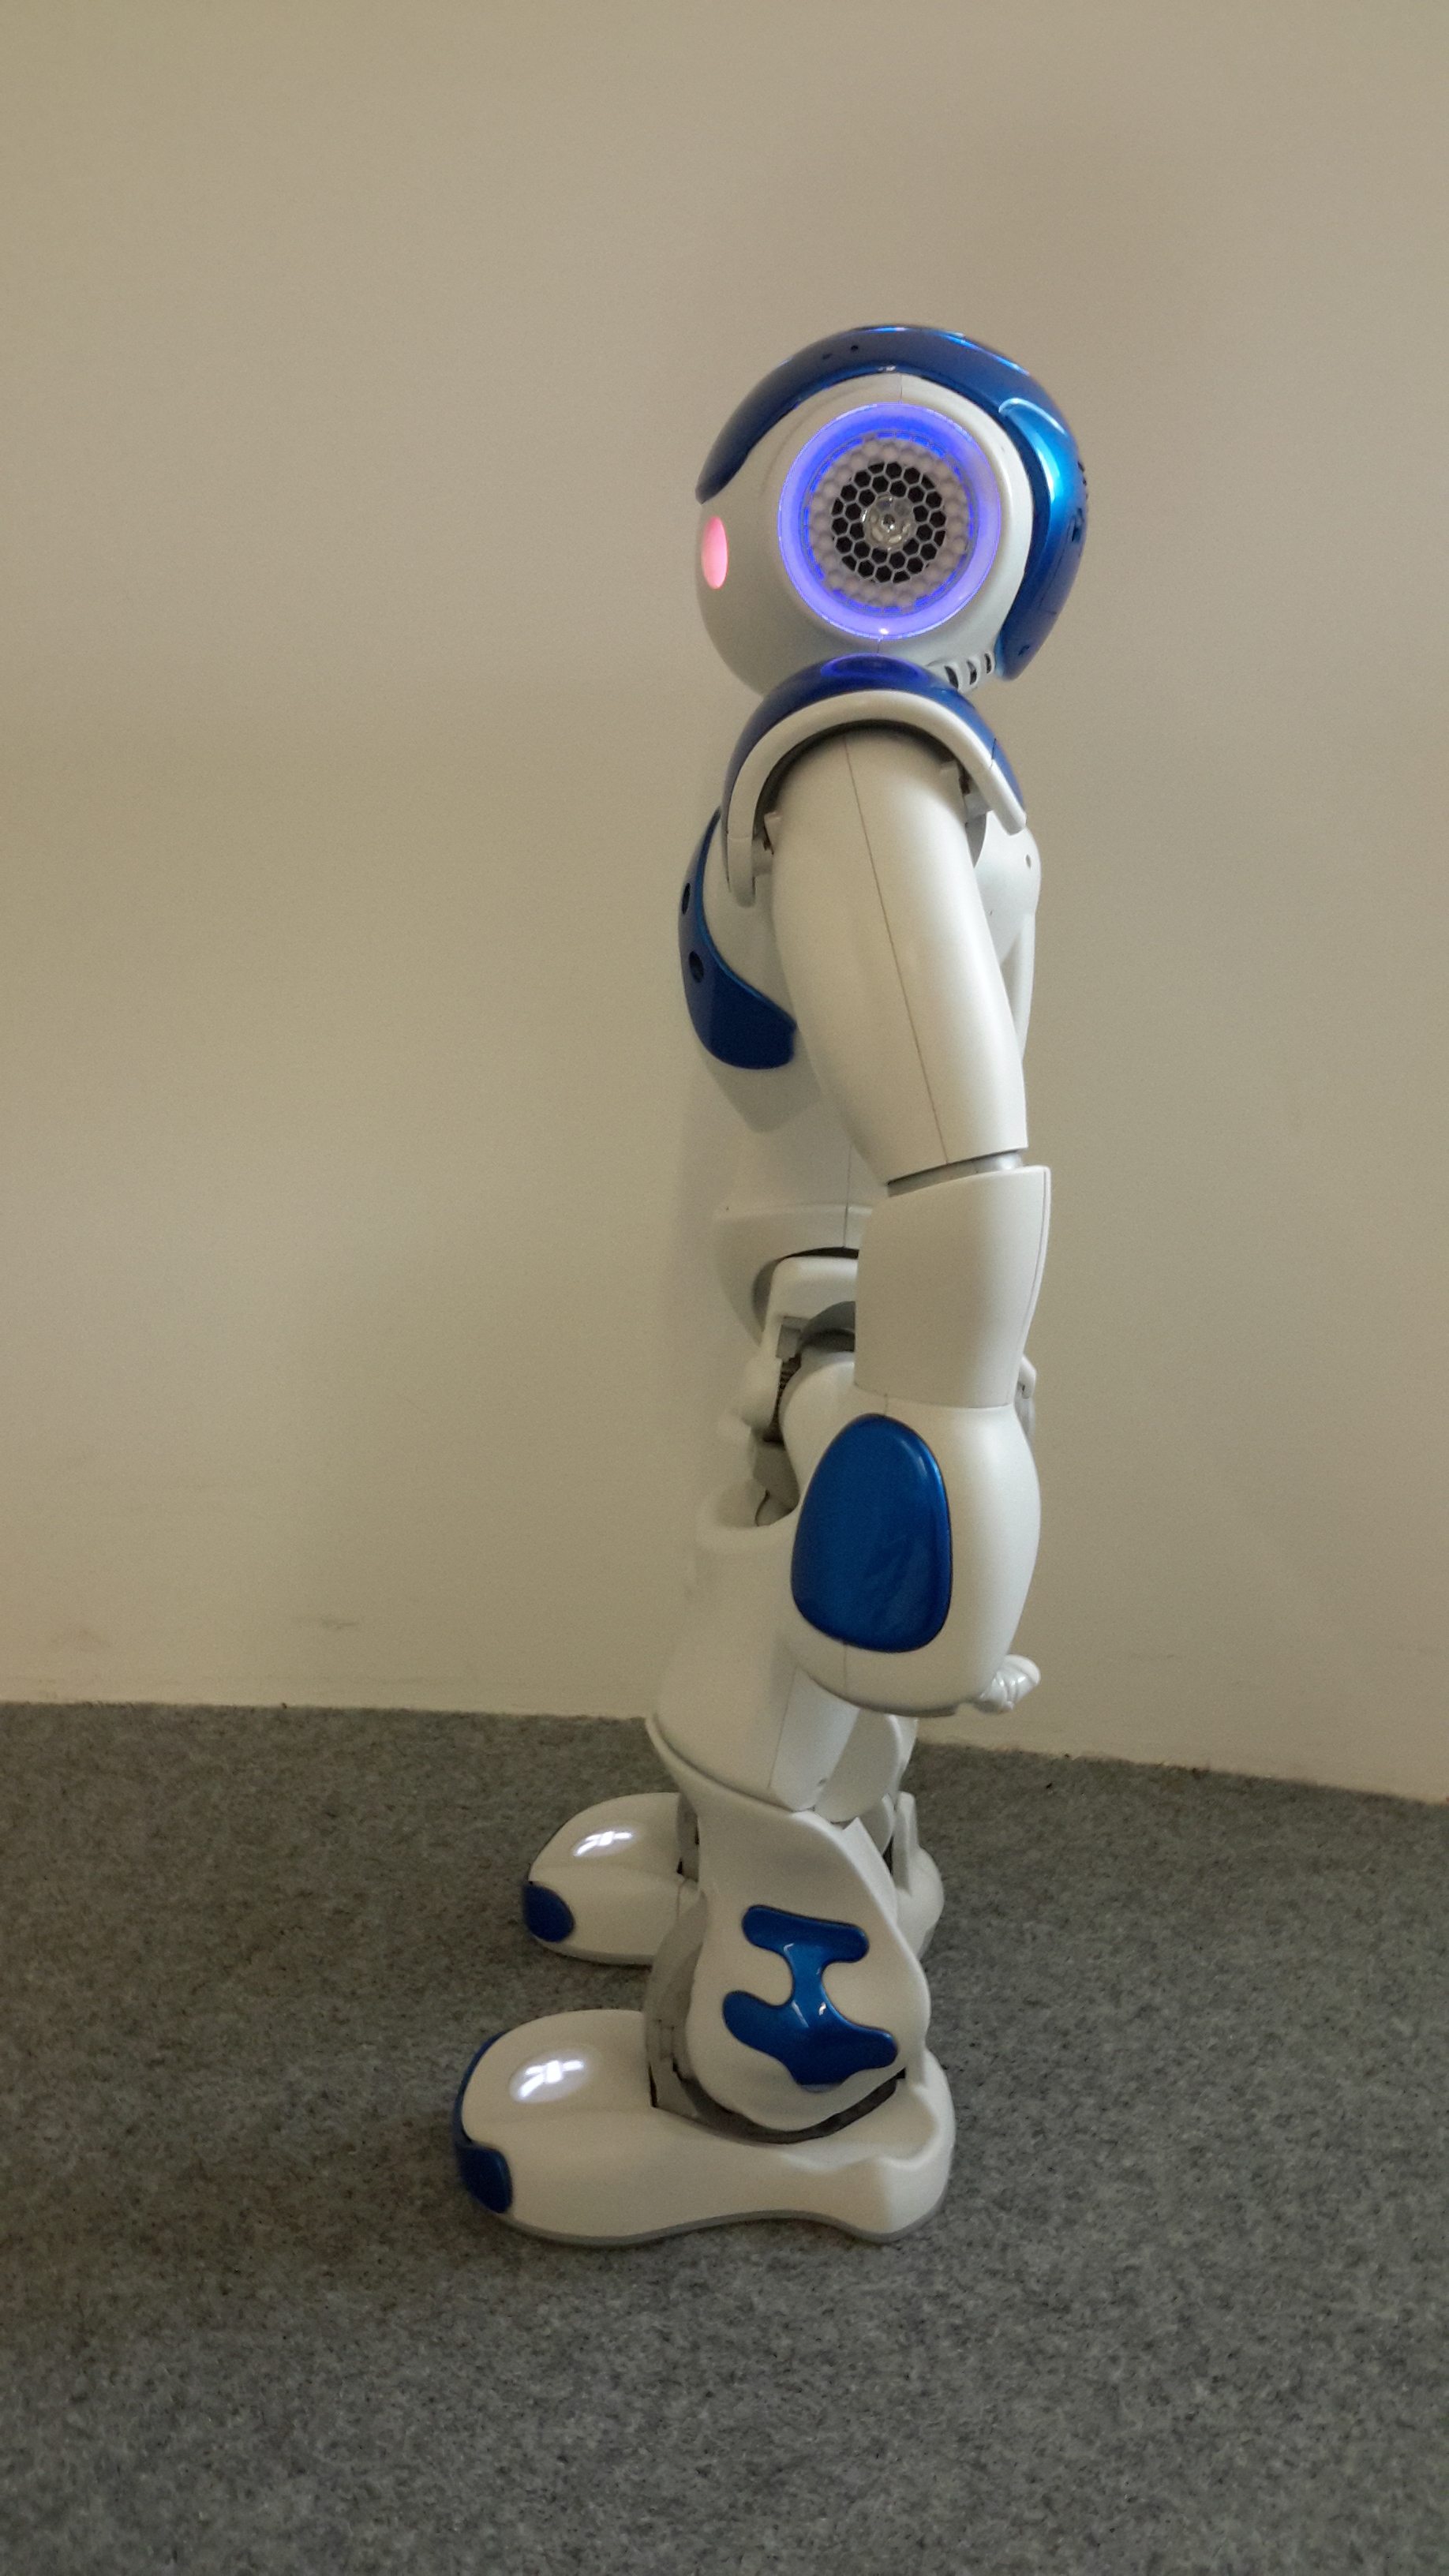
\includegraphics[width=\textwidth]{../dissertation/figures/bored.jpg}
                \caption{Bored}
                \label{fig:bored}
        \end{subfigure}
        ~ %add desired spacing between images, e. g. ~, \quad, \qquad, \hfill etc.
          %(or a blank line to force the subfigure onto a new line)
        \begin{subfigure}[b]{0.18\textwidth}
                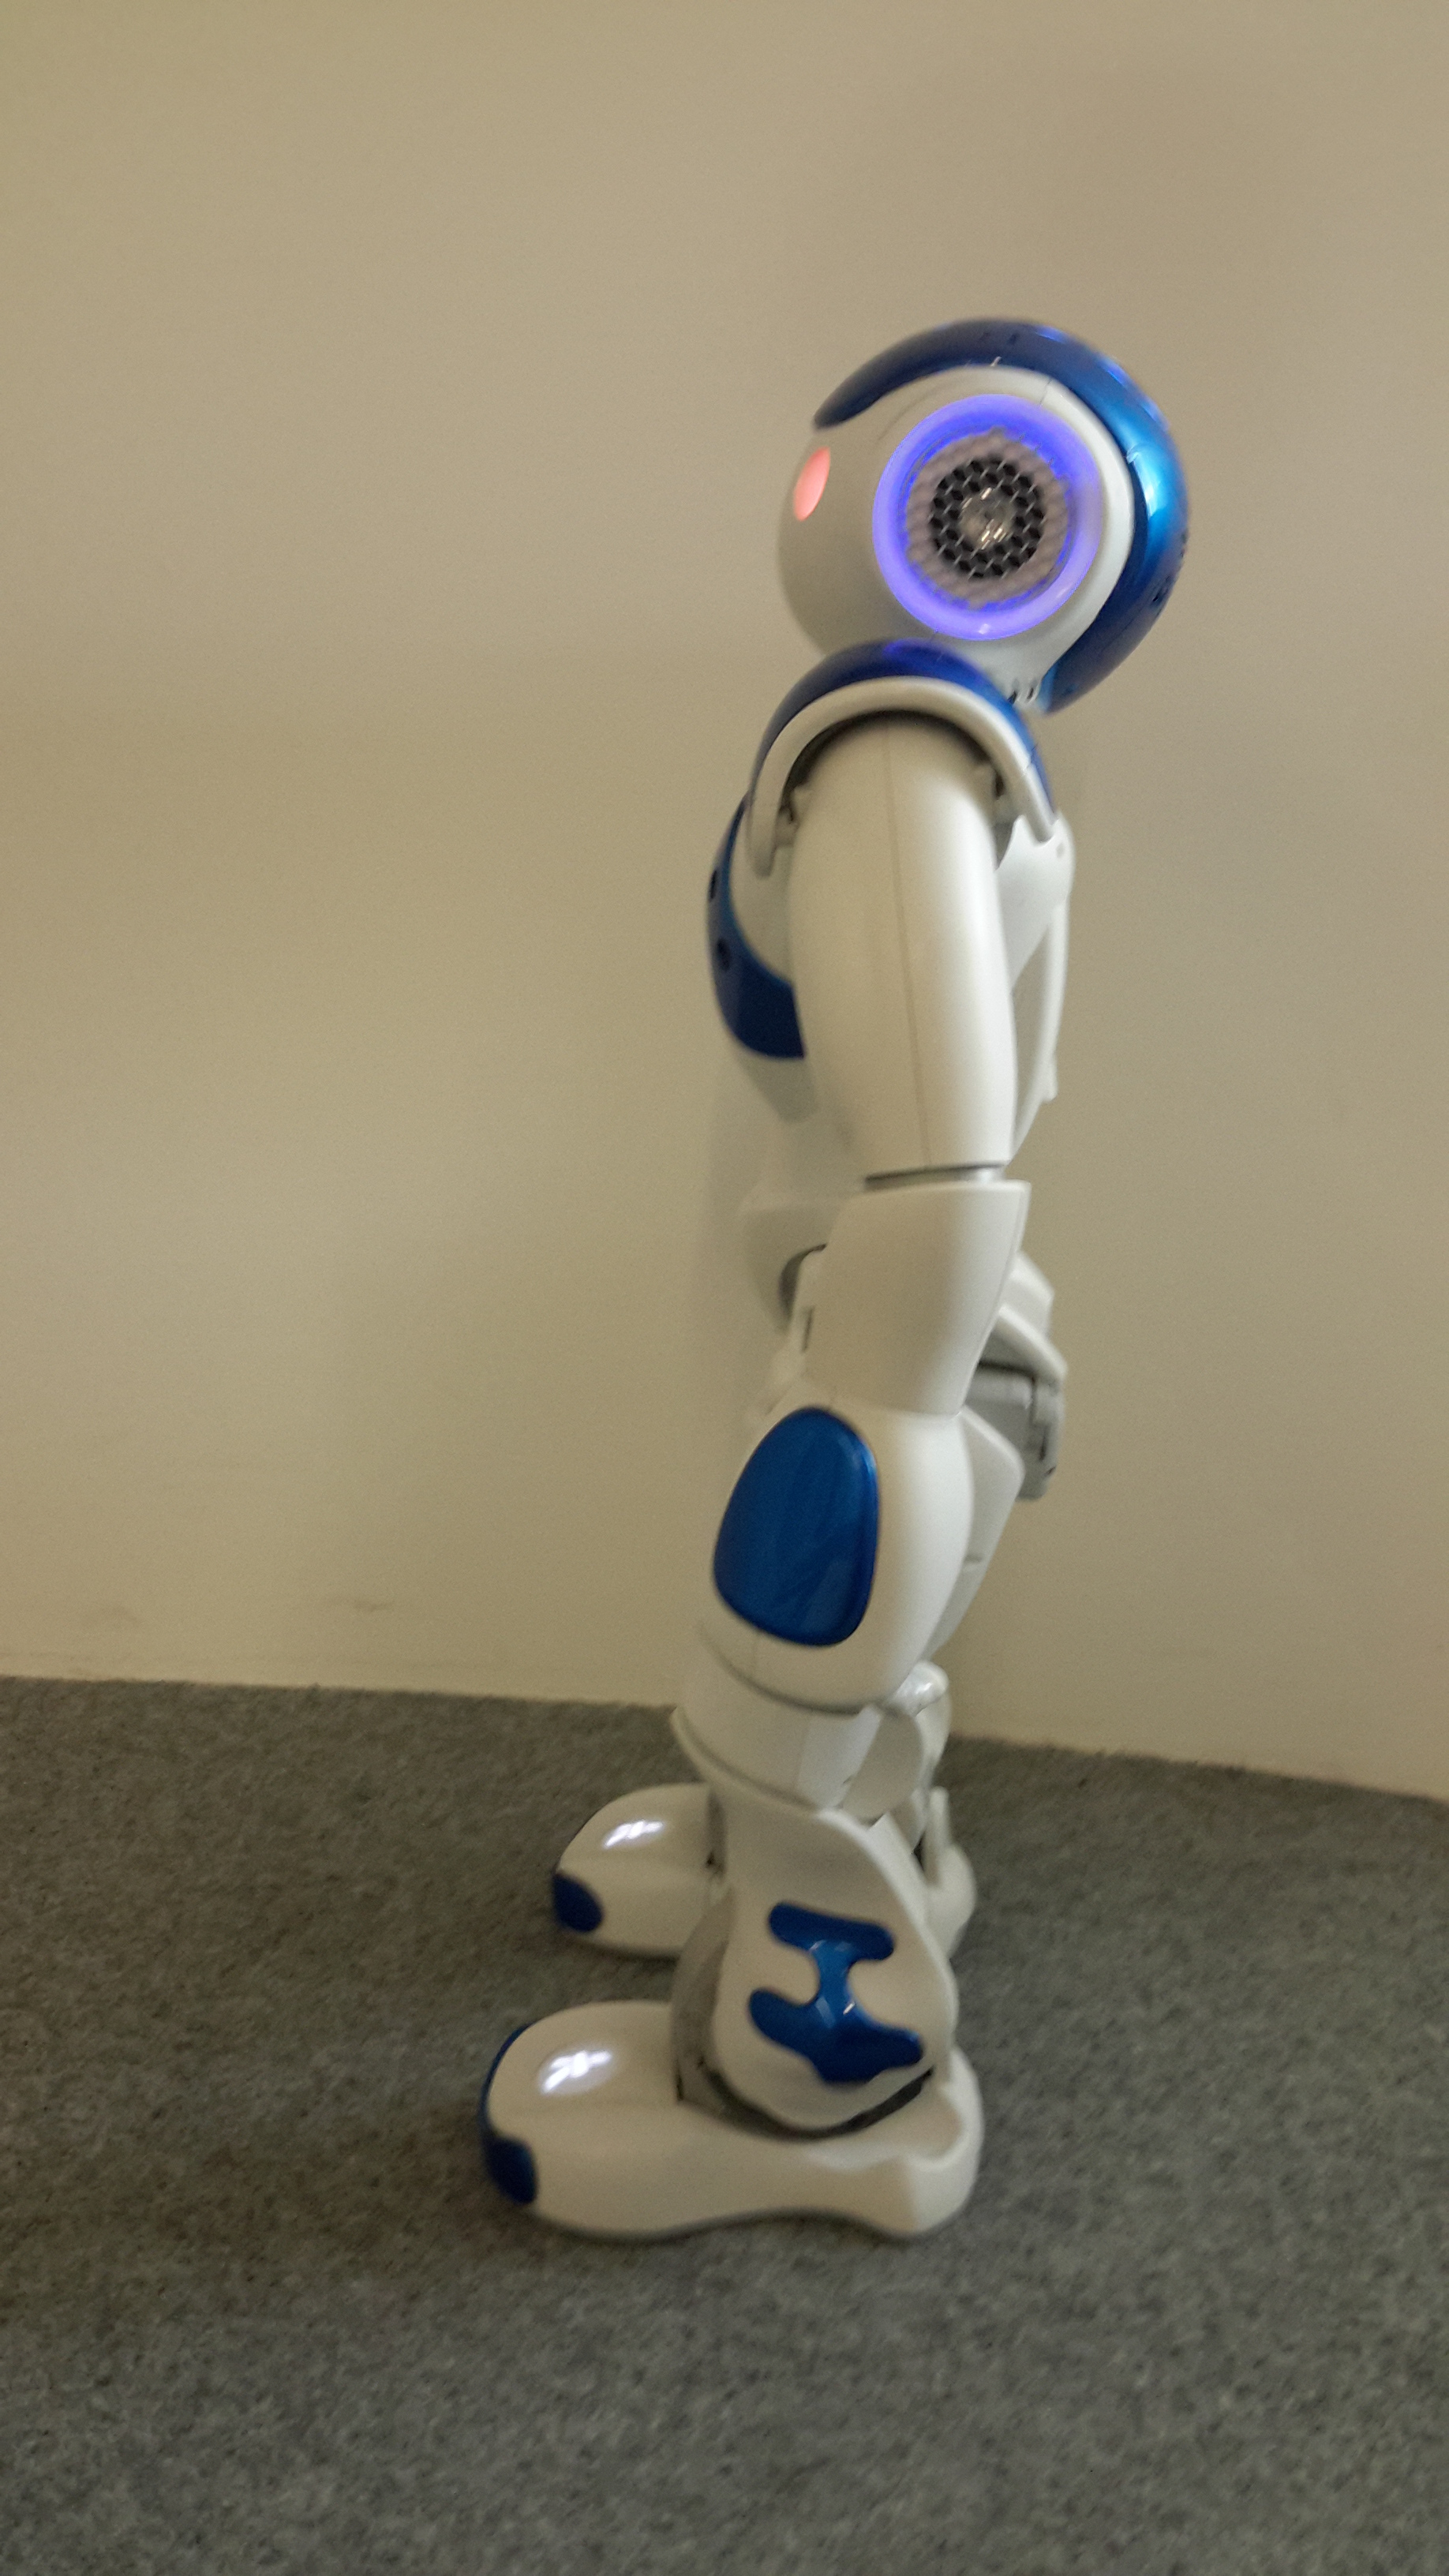
\includegraphics[width=\textwidth]{../dissertation/figures/angry.jpg}
                \caption{Angry}
                \label{fig:angry}
        \end{subfigure}
		\caption{Examples of behaviors generated by the model.}\label{fig:behaviours}
\end{figure*}

\subsection{Action manager}
Finally, this node is the interface with the robot actuators. It has been designed to encode resources such as: Head pitch, shoulders pitch and roll, speech pitch and volume, and LEDs color into the map shown in figure \ref{fig:vectMap}. In the case of the physical joints, they are distributed uniformly along the map taking into account the limitations of the joint angles. 

In this way, the result received from the \textit{emotion manager} node with range \textit{[-1,1]} is used to access the correspondent position stored in a matrix (for LEDs, pitch and volume) as well as used to modify the available joints for a certain duration of time. For instance, the shoulder roll, both right and left, are constrained between $ -76\degree $ and $ 18\degree $ were the values are defined by the \textit{valence} multiplied by a certain scale factor. The different actuators depend directly on the valence-arousal values as follows: 

\begin{itemize}
\item Head pitch: It is influenced exclusively by the arousal value. The higher the value, the higher the head position.
\item Shoulders pitch and roll: They have a pitch of +2 to -2 radians. It is exclusively modified by the valence value.
\item Speech pitch and volume: A matrix of 11x11 tuples keeps the information. It is only modified by the arousal since both parameters depend on the emotion felt \cite{banse1996acoustic}. 
\item LEDs: The same matrix dimension containing color codes was used to modify the eyes. The color is defined by an arousal since red colors are associated with high arousal whereas blue ones with low arousal \cite{elliot2014color}.
\end{itemize}

Not all actions are executed continuously during the activities. This is only the case for volume, pitch and eye color changing. The rest of the movements are performed in specific times to avoid collisions with the current activity. The result of the adaptive behavior model \footnote{https://github.com/chili-epfl/emotional-manager} is shown in figure \ref{fig:behaviours}. 

\section{Experiments}\label{sec:experiments}
Two experiences in the field has been reported. A pilot study to promote development of the design in the most appropriate directions and a data acquisition study.

\subsection{Feasibility study}

The desired outcome has been the collection of all relevant information related with the robustness of the system and the experiment protocol, including the proper detection of the most relevant features captured to assess a measurement of the level of engagement and, the implementation of an activity framework for easy addition of new activities. This study also allowed the acquisition of a ground truth model of engagement using the manual assessment by two human observers during the interaction.

\subsubsection{Experimental design}

14 children in between 5 and 6 years took part on the experiment. The children were organized in couples in order to find an emotional support with a known partner and allow a relaxed working environment.

The experimental set-up consists of the humanoid robot Nao, an external camera located between the feet of the robot and a tablet to interact with it. Moreover two observers where located away from the interaction field but with a face contact towards the children interacting to assess engagement manually. Finally, the person guiding the activity or \textit{facilitator} was located at the left of the children. The two children in front of the robot interacted during 20 min each by turns performing two activities; the original writing activity as an engaging one since intuitively is more interesting for children and a story telling as non-engaging, which was different for the two children. The words written were selected from a list provided.

\subsubsection{Measured variables} \label{measuredVariables}
During the activity the following variables has been the proximity to the region of interaction (robot and tablet), the QoM during both activities excluding the writing moments, the gaze direction, and the saliency of unexpected events. But also the time response from the end of the robot demonstration till the stylus touches the tablet and the time taken by the child to write the word.
	
Furthermore, the ground truth is one of the most important parts of the data acquisition since it will be the starting point for the results analysis. In order to acquired during the experiment, an Android ROS application was developed as a tool to help the assessment by the human observers. 

\subsection{Data acquisition experiment} \label{sec:experiment} 

After improving both the stability of the system and the experiment protocol, a second experience focused on the collection the information cited in section \ref{measuredVariables}, possibly related with the level of engagement as well as the execution of autonomous adaptive behaviors based on real-time information. In this case, 6 participants were involved in the study. A similar set-up was used together with an additional tablet to be able to select the word to write pressing a button.

\begin{figure}[h!]
        \centering
        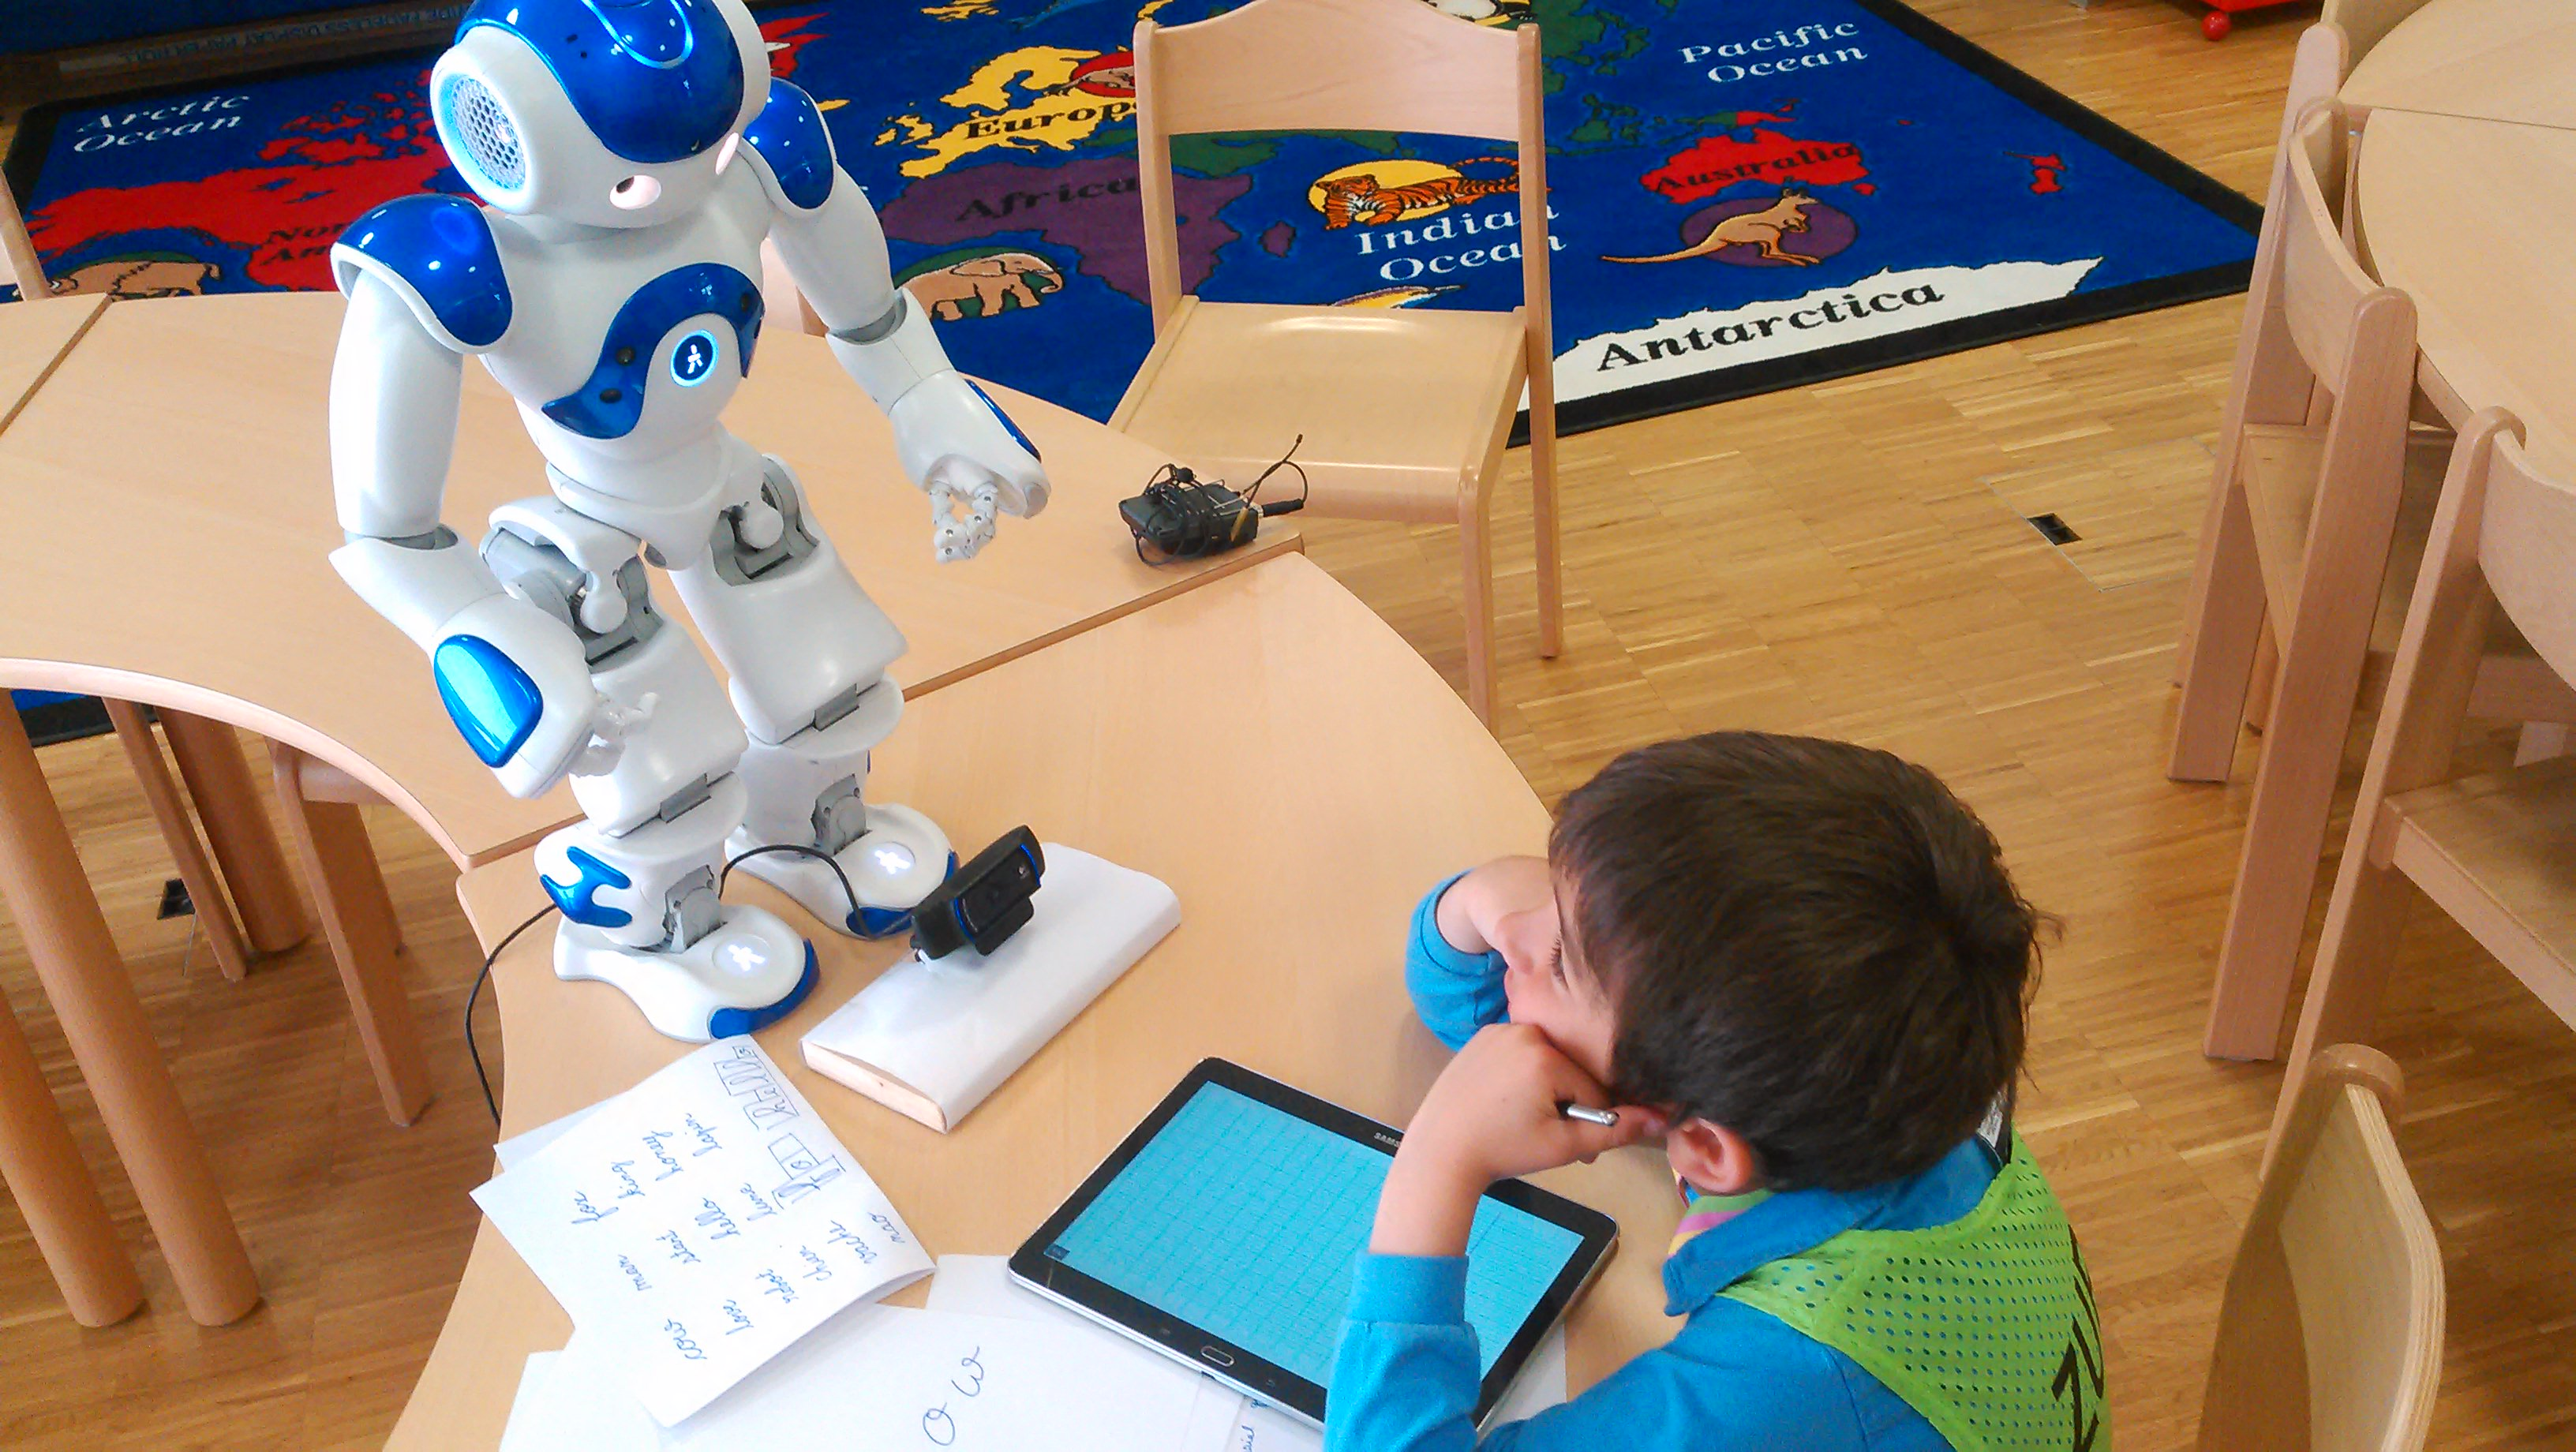
\includegraphics[width=0.3\textwidth]{../dissertation/figures/experiment.jpg}
        \caption{Redefined scenario during the data acquisition.}
        \label{fig:experiment}
\end{figure}

In this case, only one child interacted with the robot for 20 min in order to reduce the human intervention. During this time, two activities were run; the original CoWriter (writing activity) as engaging task and the story telling as non-engaging.

\section{Results}

\subsection{Measurement of engagement ground truth}
The acquisition of the grand truth was performed by two different observers that were not into the interaction field, but with direct vision towards the subjects. An example of that visual assessment is shown in figure \ref{fig:GTexample}.

\begin{figure}[h!]
        \centering
        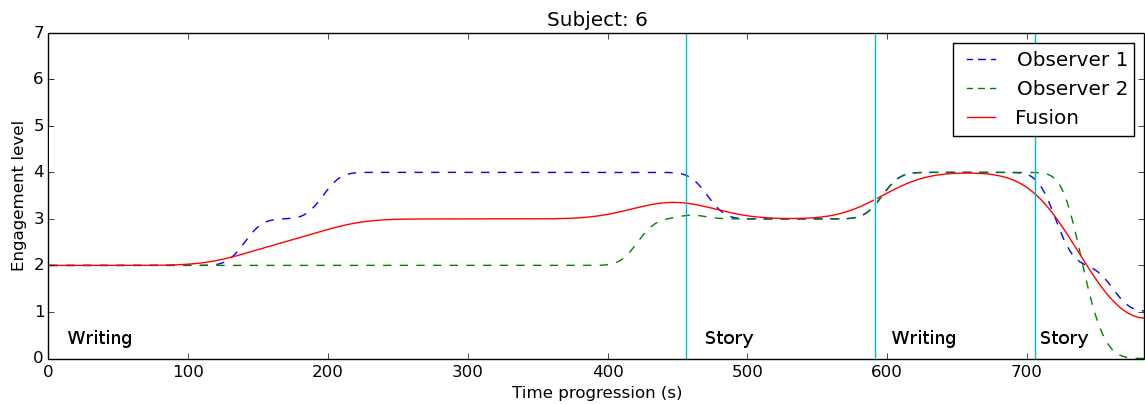
\includegraphics[width=0.45\textwidth]{../dissertation/figures/GTexample.png}
        \caption{Example of grand truth acquisition and fusion. The vertical lines indicate the activity switch.}
        \label{fig:GTexample}
\end{figure}

It is important before comparing any result to check the inter-rater reliability for the ground truth. This measurement shows if the two activities were, from the observer point of view different in terms of child engagement and how much the two human observers agreed on that. 

In order to do that, it is necessary to apply an arithmetic mean to the engagement value assessed by each of the observers taking into account each child in both CoWriter (writing) and story telling activities. After applying a Cronbach's alpha test the result obtained was $\alpha = .82$ over the 6 subjects, showing an agreement between both observers. Furthermore, a one-way between groups ANOVA has been computed to see any relevance between the assessment measurement in both activities. The result obtained was: $F[1,22] = 9.07 \quad p=.006$ which revealed that the activities lead to significantly different level of engagement.


\subsection{QoM and proximity across the two activities}
For QoM and proximity greater means correspond to the writing activity as we can see in figures \ref{fig:meanMov} and \ref{fig:meanProx}. It leads to the assertion that QoM and proximity are directly related at least, with an active or passive activity.

Since the population studied does not exceed the 6 participants, we can not assume the data is normally distributed thus a T-test makes an estimation of the deviation. The results obtained for both features shows a marginal significance in the QoM $ (t(df=10)= 2.0964, p = 0.06245) $ and significance\footnote{There is significance if $p<0.05$ and marginal significance if $p<0.1$} for the proximity measurement $(t(df=9.7406)= -2.8338, p = 0.01818) $. In addition, mean and standard deviation are shown in table \ref{tab:pvalues}.

\begin{figure*}
        \centering        
        \begin{subfigure}[b]{0.35\textwidth}
                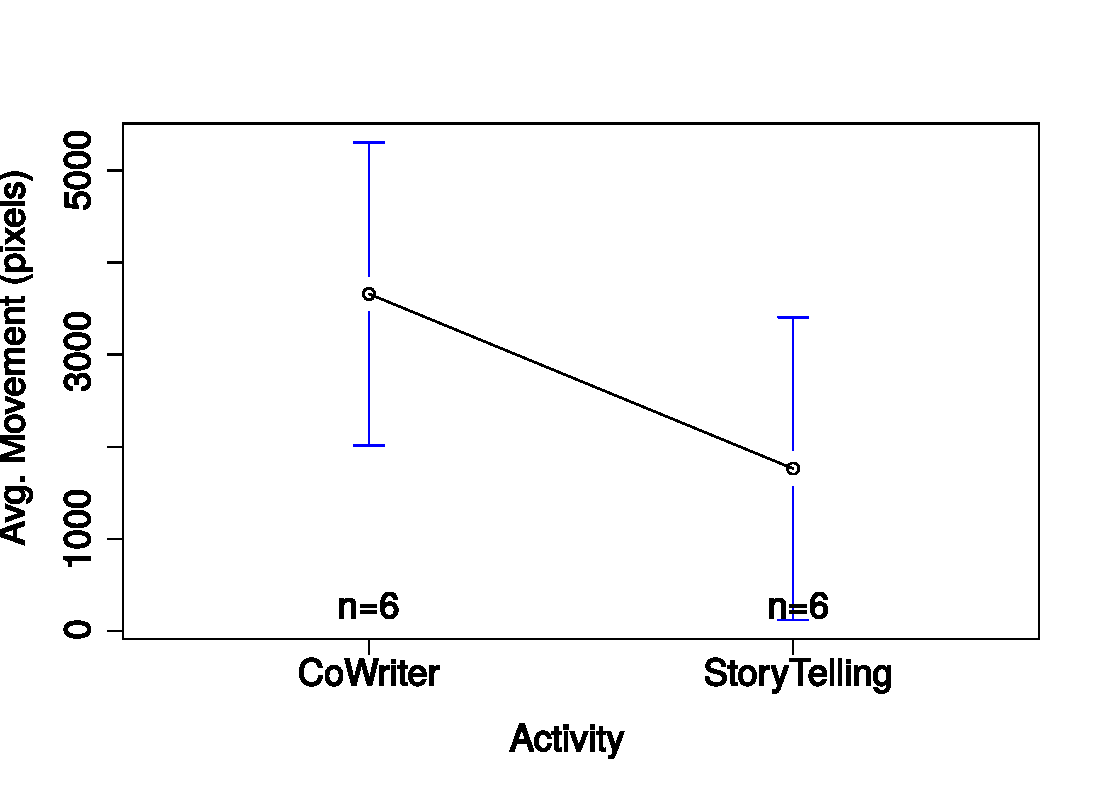
\includegraphics[width=\textwidth]{../dissertation/figures/AvgMovement.pdf}
                \caption{QoM}
                \label{fig:meanMov}
        \end{subfigure}
        %add desired spacing between images, e. g. ~, \quad, \qquad, \hfill etc.
          %(or a blank line to force the subfigure onto a new line)
        \begin{subfigure}[b]{0.35\textwidth}
                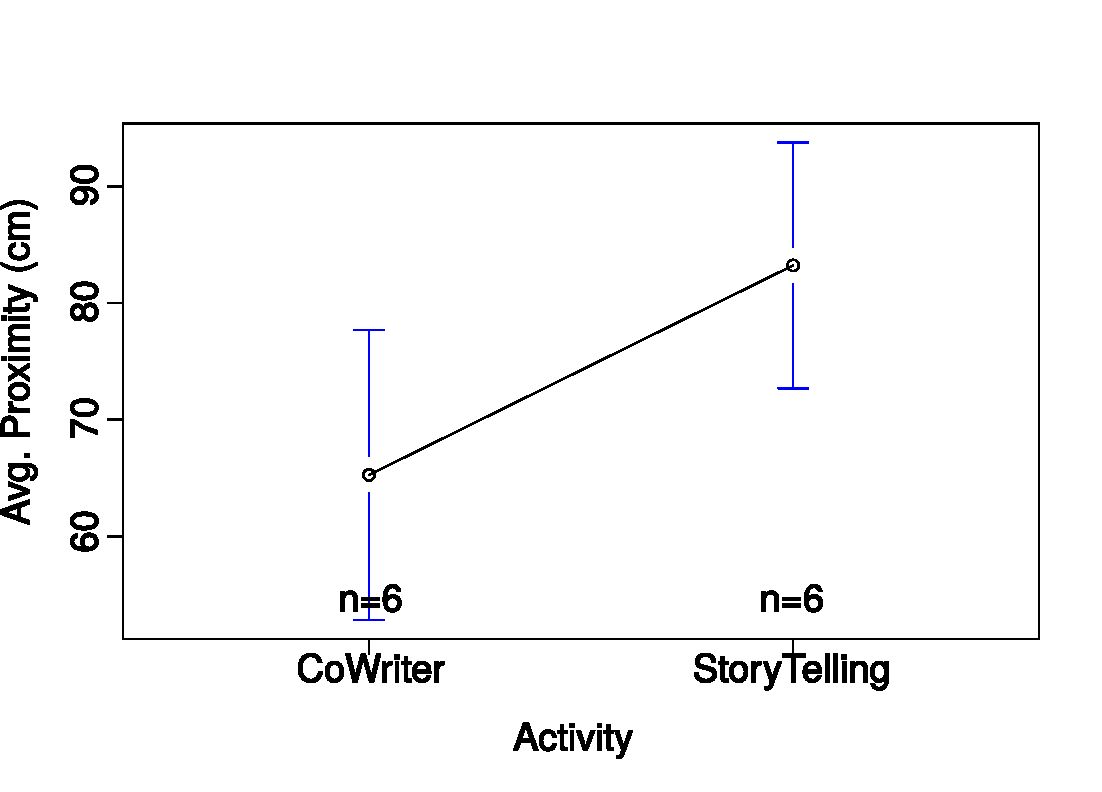
\includegraphics[width=\textwidth]{../dissertation/figures/AvgProximity.pdf} 
                \caption{Proximity}
                \label{fig:meanProx}
        \end{subfigure}%
        		
        \begin{subfigure}[b]{0.35\textwidth}
                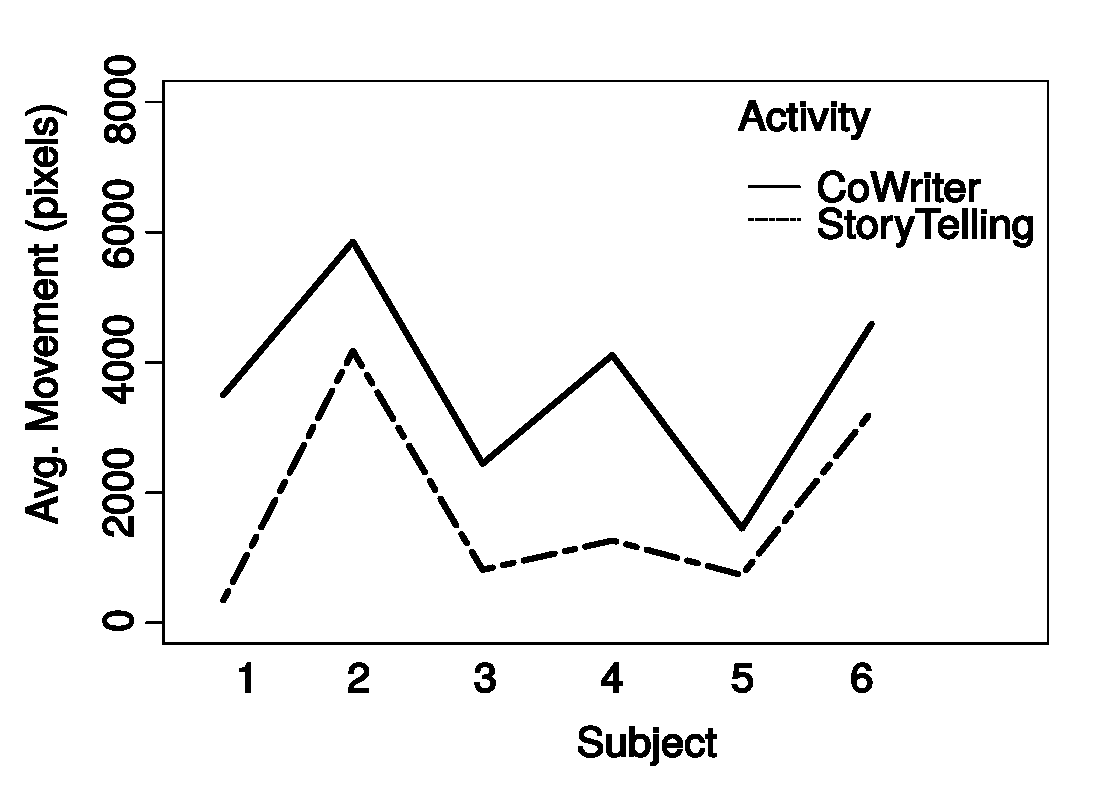
\includegraphics[width=\textwidth]{../dissertation/figures/AvgMovement2.pdf}
                \caption{QoM}
                \label{fig:anovaMov}
        \end{subfigure}
         %add desired spacing between images, e. g. ~, \quad, \qquad, \hfill etc.
          %(or a blank line to force the subfigure onto a new line)
        \begin{subfigure}[b]{0.35\textwidth}
                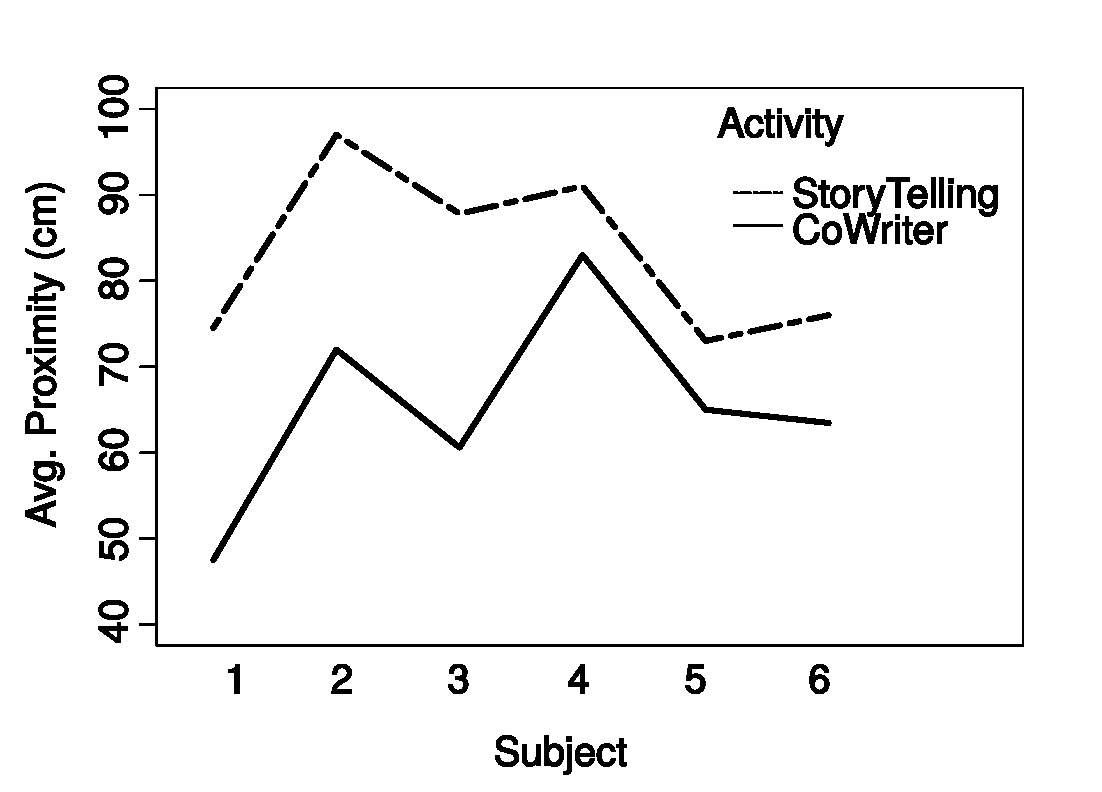
\includegraphics[width=\textwidth]{../dissertation/figures/AvgProximity2.pdf}
                \caption{proximity}
                \label{fig:anovaProx}
        \end{subfigure}
		\caption{Mean plots (a)(b) and inter-subject measurement variability (c)(d)}
\end{figure*}


\begin{table}[h!]
\centering
\begin{tabular}{l|l|l|l|l}
          & \multicolumn{2}{c|}{\textbf{Writing}}                               & \multicolumn{2}{c|}{\textbf{Story telling}}                        \\ \cline{2-5} 
          & \multicolumn{1}{c|}{$\mu$} & \multicolumn{1}{c|}{$\sigma$} & \multicolumn{1}{c|}{$\mu$} & \multicolumn{1}{c}{$\sigma$} \\ \hline
\textbf{QoM}  &          3658.78                  &         1567.51                      &              1763.05              &              1564.94                \\ \hline
\textbf{Proximity} &      65.2600                      &           11.837                    &          83.2167                  &              10.0400                
\end{tabular}
\caption{T-test mean, $\mu$ and standard deviation, $\sigma$.}
\label{tab:pvalues}
\end{table}


However, a more accurate measurement across groups is performed using a one way repeated measures ANOVA since it is a single group (6 subjects) on which we have measured the QoM and the proximity a few times (for writing and story telling activities) during the same amount of time. The results shown a significance \textit{F[1,115]=21.01, p=1.17e-05} being $ p<.001 $ for proximity and no significance for QoM \textit{F[1,286]=0.729, p=0.394}. Therefore, the proximity to the interaction field is a good indicator of the child's engagement in an active activity. 

In addition, the results are consistent with the lines shown in figures \ref{fig:anovaMov} and \ref{fig:anovaProx}, where in both cases the two groups are rather close together. Actually, the within subject test indicates that there is a significant relation between subjects, in other words, the groups do change between subjects but preserve a similar difference between activities.

Finally, in figure \ref{fig:avgProximity} we can see the average normalized proximity between the subjects over time, where the vertical lines indicate the story telling starting point in each case. In 5 over 6 subjects there is a tendency to decrease the proximity to the field of interaction right after the execution of the story telling activity.

\begin{figure}[h!]
        \centering
        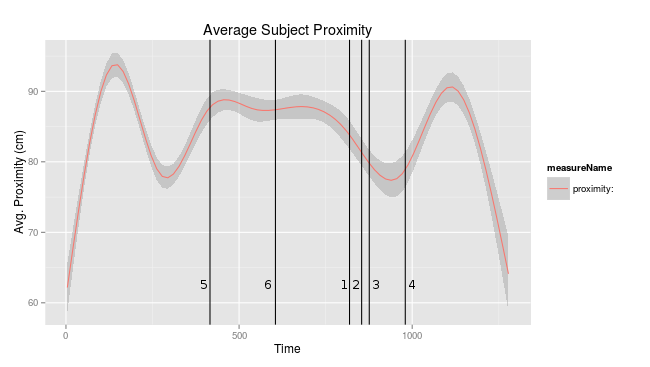
\includegraphics[width=0.5\textwidth]{../dissertation/figures/avgProximity.png}
        \caption{Average proximity measurement between subjects. The vertical lines indicate the story telling starting point.}
        \label{fig:avgProximity}
\end{figure}

\subsection{The gaze information}

The gaze direction turned to be interesting from the interaction point of view, being able to show the amount of intervention (figure \ref{fig:gaze}) needed from the facilitator sitting on the left of the subject, against the visual contact towards the field of interaction (robot and tablet) for a single subject.
\begin{figure}[!htb]
	\centering
	\begin{tikzpicture}[>=latex]
		\node[inner sep=0pt] (xtion) at (0,0) {
		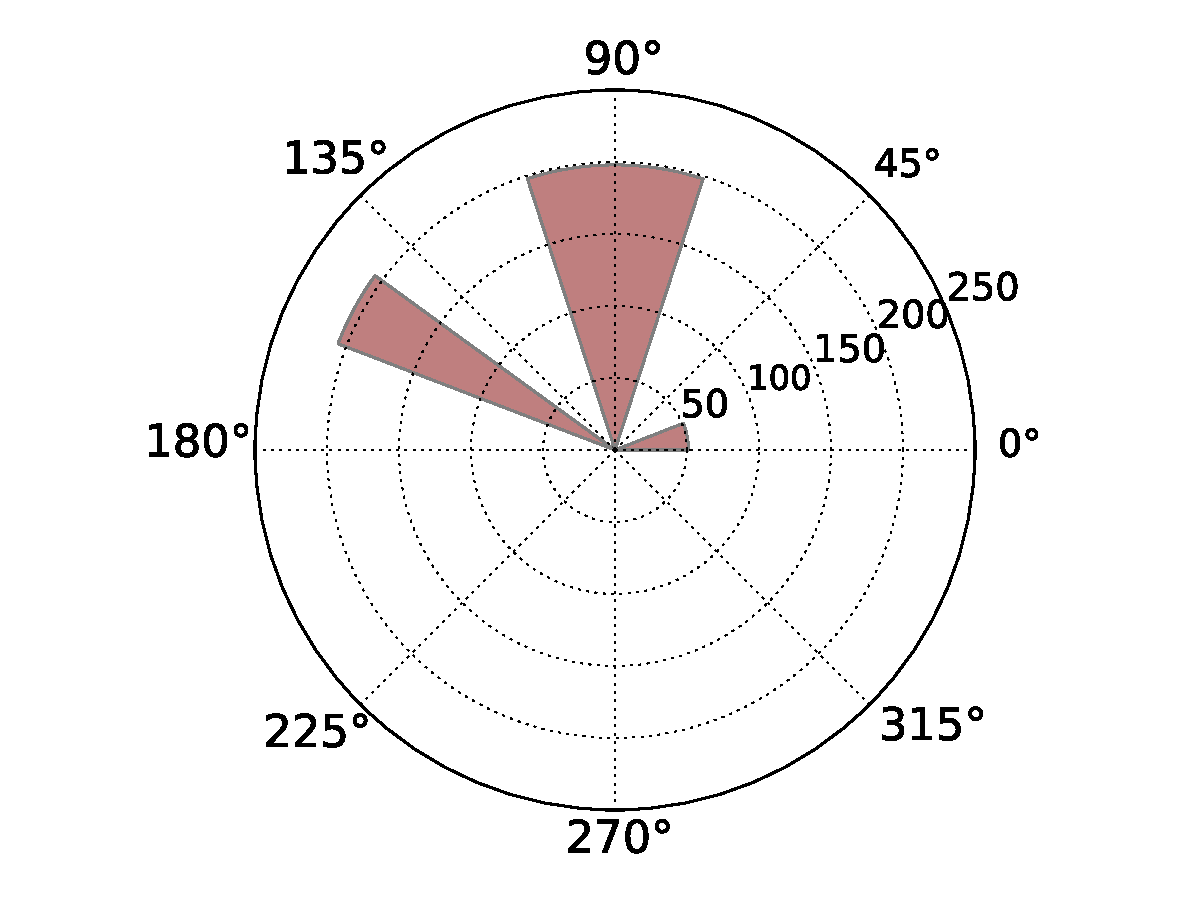
\includegraphics[width=0.3\textwidth]{../dissertation/figures/gaze.pdf}};	
		\node[black, text width=2cm] at (0.74,2) {		
		Robot	
		};		
		\node[black, text width=2cm] at (-1.3,0.5) {		
		Facilitator	
		};				
	\end{tikzpicture}
    \caption{A Subject's mean gaze direction in time.}
    \label{fig:gaze}
\end{figure}
We can hypothesize that during the writing activity the children look more to the left and less to the robot in comparison with the story telling activity. Furthermore, in order to test how likely it is that an observed distribution is due to chance or not, a Pearson's Chi-squared has been computed. The result $(\chi^2(df=6,  N=537.75), p-value < 2.2e-16)$ shows a tiny chance. Secondly, the residuals of the Chi-squared test comparing the observed data summarized in table \ref{tab:chi} verifies the hypothesis formulated previously based on one subject observation.

\begin{table}[h!]
\small
\centering
\begin{tabular}{l|l|l|l|l}
 		 		  & \textbf{Down} & \textbf{Left}	& \textbf{Right} & \textbf{Robot}	    \\ \hline	
 \textbf{Wt} &  102(3.481) & 2965(4.455) & 35(-0.149)  &  993(-7.701)    \\ \hline
 \textbf{St}    &    0(-1.154) & 215(-10.68)      & 6(0.359)      & 371(18.477)
\end{tabular}
\caption{Chi-square test for writing (wr) and story (st).}
\label{tab:chi}
\end{table}

As we hypothesize, the users tend to change their gaze direction towards the \textit{facilitator} located on the left and to the FoI during the writing activity whereas the gaze focus during the story telling activity is on the robot and facilitator, which is supposed not to be required. It suggests a future improvement towards a more independent system specially in the writing activity.

\section{CONCLUSIONS AND FUTURE WORKS}

The challenges involved in developing such a technology which have been addressed in this work include a real-time robot adaptive behavior based on face features, an engagement assessment using visual and non-visual features and an improvement of the user experience within the CoWriter project by the addition of new functionalities. The use of the child's face proximity to the field of interaction as an indicator of engagement in the specific context of the writing and the story telling activities is significant since in most of the cases the proximity decreases during a non-engaging and passive task. Furthermore, the gaze direction has been very useful in the quantification of the facilitator involvement in the activity. It proves that the percentage of implication of the person helping during the activity time, specially in the writing task is high. 

Finally, the adaptive behavior model proposed based on on-line acquisition of user information such as proximity, QoM and gaze direction among others, seems to be a reasonable way to model a rich set of behaviors according to the specific context of the situation. 


%%%%%%%%%%%%%%%%%%%%%%%%%%%%%%%%%%%%%%%%%%%%%%%%%%%%%%%%%%%%%%%%%%%%%%%%%%%%%%%%

Additional work needs to be done in two aspects in particular: The robot independence from the facilitator and the on-line engagement detection for practical use.  

The independence of the system without requiring any human intervention is the most complex and challenging one. It is necessary to design interaction protocols with a continuous and quick feedback to the user. A way to do that is to provide short-term events such as a gesture generation according to the context of activity. For instance, a good performance in the writing of a word, should lead to show a positive gesture from the robot that would reinforce the children interacting.

\addtolength{\textheight}{-14.5cm}

\bibliographystyle{ieeetr}

\bibliography{tex/refs.bib}

\end{document}
